\chapter{Superconduttività}
La superconduttività fu scoperta per la prima volta nel 1911 da Kamerlingh Onnes durante uno studio riguardante la resistività dei metalli puri a bassa temperatura. Onnes osservò che la resistività del campione di mercurio oggetto di studio scendeva drasticamente a temperature sotto i $\SI{4.2}{\kelvin}$, come mostrato in figura \ref{fig: resistività Hg}. 
\begin{figure}[h]
    \centering
    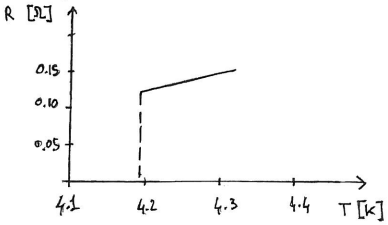
\includegraphics[width=0.5\linewidth]{Immagini - Capitolo 2/resistività Hg.png}
    \caption{andamento della resistenza $R$ del mercurio in funzione della temperatura.}
    \label{fig: resistività Hg}
\end{figure}

Valori di resistenza anche molto piccoli possono essere misurati attraverso la diminuzione della corrente in un conduttore ad anello. La corrente in quest'ultimo dovrebbe diminuire secondo la legge 
\begin{equation}
    i(t) = I_0e^{-Rt/L},
\end{equation}
dove $L$ è l'induttanza dell'anello. Dagli esperimenti di questo tipo si può concludere che la resistività crolla di almeno sedici ordini di grandezza scendendo al di sotto di una certa temperatura critica $T_c$, entrando nel regime di superconduzione. In queste condizioni la corrente scorre senza subire fenomeni di dissipazione dimostrando che la resistività di un superconduttore non è solo piccola ma essenzialmente nulla. La temperatura critica, o di transizione, dipende quasi esclusivamente dalla natura del superconduttore e varia in un range molto ampio, alcuni esempi sono elencati in tabella \ref{tab: esempi di temperature critiche}.
\begin{table}[h]
    \centering
    \begin{tabular}{|c|c|}
        \hline
         Elemento & $T_c\,[\mathrm{K}]$ \\ \hline
         $\ce{Al}$ & 1.19 \\
         $\ce{Hg}$ & 4.15 \\ 
         $\ce{Ga}$ & 1.09 \\ 
         $\ce{HgBa2Ca2Cu3O_x}$ & 135 \\ \hline
    \end{tabular}
    \caption{esempi di temperature critiche di alcuni elementi.}
    \label{tab: esempi di temperature critiche}
\end{table}
Infatti, la struttura reticolare non è rilevante per determinare quali materiali possono essere superconduttori: cristalli puri, leghe e metalli amorfi possiedono proprietà di superconduzione; persino il silicio diventa un superconduttore, seppur ad alta pressione e bassa temperatura. Tipicamente, i metalli puri entrano in regime di conduzione al di sotto dei $\SI{10}{\kelvin}$, mentre i composti metallici attorno ai $\SI{20}{\kelvin}$. Ottimi conduttori come l'oro, il rame e l'argento non entrano in regime di conduttore fino a temperature nell'ordine del kelvin. In generale, nemmeno le impurità influiscono sul comportamento di un superconduttore, a parte le impurità magnetiche. Queste ultime infatti tendono ad intrappolare elettroni e ad annullare le proprietà di superconduttività, un fenomeno che prende il nome di effetto Kondo. Tipicamente, la transizione di fase a supeconduttore avviene senza un cambiamento della struttura reticolare. Inoltre, materiali composti possono essere superconduttori sebbene i loro singoli costituenti rimangano nel regime di conduzione normale. Risulta invece essere rilevante il volume atomico, infatti normalmente materiali composti da volumi atomici grandi sono sfavoriti ad entrare in superconduzione. 

\section{Effetto Meissner-Ochsenfeld}
Nel 1933, Meissner e Ochsenfeld scoprirono che la transizione al regime di superconduzione non corrisponde solo alla quasi totale assenza di resistenza, ma anche alla comparsa di un comportamento diamagnetico ideale. Questo effetto sta anche alla base della distinzione tra un superconduttore e un conduttore ideale con resistenza nulla. Dalla legge di Faraday
\begin{equation}
    \frac{\p \Phi(t)}{\p t} = -\oint_{\p\Sigma}\vE \cdot d\bm{\Sigma},
\end{equation}
si ha che la variazione di flusso di campo magnetico attraverso un cammino chiuso induce un campo elettrico $\vE$. Tuttavia, in un conduttore ideale e in un superconduttore la resistenza è nulla, per cui non vi possono essere differenze di potenziale, quindi un campo elettrico, per cui il campo magnetico $\vB$ risulta stazionario all'interno di essi. Nella pratica, la schermatura del campo magnetico esterno avviene grazie alla formazioni di correnti superficiali di superconduzione.

Si considerino quindi due esperimenti in cui si confronta il comportamento di un conduttore ideale con quello di un superconduttore. Dato un campo magnetico esterno $\vB_a$, si indica con $t_0$ l'istante in cui viene raggiunto il regime di superconduzione. Nel primo esperimento, mostrato sempre in figura \ref{fig: effetto M-O I e II}, per entrambi i campioni il campo magnetico non può penetrare al loro interno. Dato che la resistenza è nulla, la corrente schermante in entrambi i casi non si dissipa fino alla scomparsa del campo magnetico esterno. Nel secondo esperimento, mostrato in figura \ref{fig: effetto M-O I e II}, il campo magnetico viene acceso prima dell'istante $t_0$, il quale non viene schermato da entrambi i campioni. Tuttavia, dopo l'istante $t_0$, il campo magnetico viene schermato solo dal superconduttore, mentre il conduttore ideale continua ad essere attraversato da esso. Quando poi il campo magnetico viene spento, il conduttore ideale rimane magnetizzato, mentre il superconduttore non presenta alcun segno della presenza di $\vB_a$. Questa differenza nel comportamento dei due campioni è proprio l'effetto di Meissner-Ochsenfeld. 
\begin{figure}[h]
    \centering
    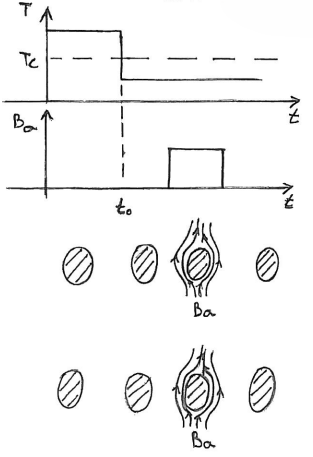
\includegraphics[width=0.4\linewidth]{Immagini - Capitolo 2/effetto M-O I.png}
    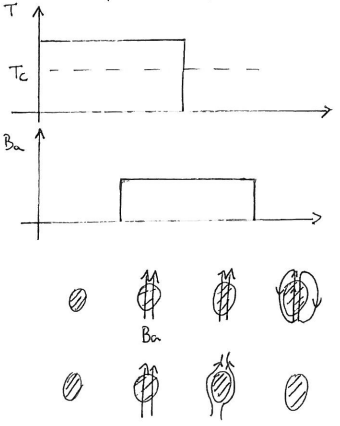
\includegraphics[width=0.45\linewidth]{Immagini - Capitolo 2/effetto M-O II.png}
    \caption{visualizzazione dell'effetto Meissner-Ochsenfeld (la prima riga si riferisce al conduttore ideale, la seconda al superconduttore).}
    \label{fig: effetto M-O I e II}
\end{figure}

Nel caso di un conduttore ad anello, la situazione non è molto differente. Il campo magnetico viene espulso dall'interno del superconduttore, ma si instaurano delle correnti schermanti sulla superficie che persistono anche quando il campo magnetico cessa di esserci, come mostrato in figura \ref{fig: effetto M-O III}. Si noti comunque come il flusso di campo magnetico all'interno dell'anello non viene respinto dal superconduttore.
\begin{figure}[h]
    \centering
    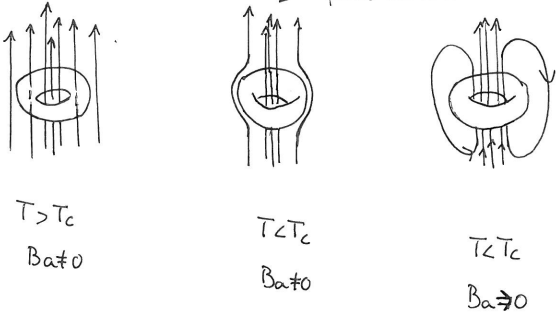
\includegraphics[width=0.5\linewidth]{Immagini - Capitolo 2/effetto M-O III.png}
    \caption{effetto Meissner-Ochsenfeld in un superconduttore ad anello.}
    \label{fig: effetto M-O III}
\end{figure}

Ad ogni modo, un forte campo magnetico esterno può distruggere la superconduttività, ristabilendo lo stato normale di conduzione. A seconda del tipo di transizione, si possono distinguere due tipi di superconduttori, quelli di tipo I e quelli di tipo II.

\section{Superconduttori di tipo I}
Il comportamento di un superconduttore di tipo I immerso in campo magnetico esterno $\vB_a$ è mostrato in figura \ref{fig: SC tipo I}, dove si osserva un valore critico $\vB_c$ del campo magnetico che sancisce il confine tra il regime di conduzione normale e quello di superconduzione. Il campo magnetico interno al superconduttore può essere scritto 
\begin{equation}
    B_i = B_a + \mu_0M = \mu_0(H_a + M),
\end{equation}
dove $\mu_0$ è il coefficiente di suscettività magnetica nel vuoto. Per temperature $T < T_c$ si ha che $B_i = 0$ se e solo se
\begin{equation}
    \chi = \mu_0\frac{\p M}{\p B_a}\bigg|_{B_a = 0} = \frac{\mu_0M}{B_a} = -1.
\end{equation}
Questo risultato esprime il fatto che i superconduttori di tipo I sono diamagneti ideali. Se il campo magnetico esterno viene incrementato, la schermatura si ``rompe'' al valore critico $B_c$ e il conduttore ritorna allo stato normale di conduzione. Il valore del campo magnetico critico dipende dalla temperatura del materiale, in particolare segue la legge empirica
\begin{equation}
\label{eq: valore cricito Bc nei SC di tipo I}
    B_c(T) = B_c(0)\bigg[1 - \bigg(\frac{T}{T_c}\bigg)^2\bigg].
\end{equation}
\begin{figure}[h]
    \centering
    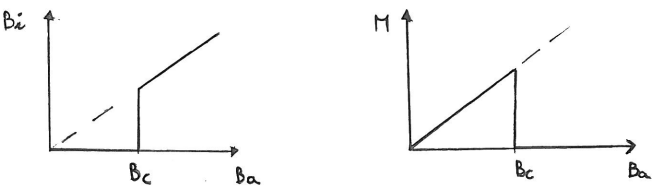
\includegraphics[width=0.7\linewidth]{Immagini - Capitolo 2/SC tipo I.png}
    \caption{andamento in funzione di $B_a$: (i) del campo magnetico interno al superconduttore $\vB_i$; (ii) della magnetizzazione $M$.}
    \label{fig: SC tipo I}
\end{figure}

Analogamente, quando un superconduttore è percorso da una corrente elettrica $I > I_c$, il campione transisce al regime normale. Per determinare il valore critico della corrente $I_c$ si deve considerare che in nessuna regione del superconduttore la corrente può superare $I_c$. Non ha importanza che questa sia la corrente di schermaggio o causata da un generatore di corrente ai capi del superconduttore. Si considera quindi un filo di raggio $R$, il campo magnetico sulla superficie del cavo è
\begin{equation}
    B = \frac{\mu_0I}{2\pi R},
\end{equation}
di conseguenza la corrente critica è semplicemente data da
\begin{equation}
    I_c = \frac{2\pi RB_c}{\mu_0},
\end{equation}
da cui si nota la proporzionalità con la circonferenza del filo, e non con la sua area. Alcuni esempi di superconduttori di tipo I sono il piombo, il mercurio e l'alluminio.

\section{Superconduttori di tipo II}
Come in quelli di tipo I, il campo magnetico viene completamente espulso fino a quando il valore del campo è inferiore ad un primo valore critico $B_{c_1}$. A valori superiori si formano canali di conduttore normale in regime di conduzione normale che permettono al campo esterno $\vB_a$ di penetrare nella forma di filamenti sottili, chiamati linee di flusso o vortici di superconduttori.
\begin{obs}
    Si vedrà che il flusso del campo magnetico, per ognuno di questi filamenti, o equivalentemente la circuitazione delle supercorrenti, non è quantizzata.
\end{obs}
L'esistenza di due tipi di superconduttore è legata all'energia di interfaccia tra regimi normale e di superconduzione che è positiva in quelli di tipo I, ma negativa in quelli di tipo II, favorendo così la formazione regioni di conduzione normale all'interno dei secondi. Il campo magnetico e la magnetizzazione all'interno di un superconduttore di tipo II, in funzione del campo magnetico applicato, hanno l'andamento la forma mostrata in figura \ref{fig: SC tipo II}.
\begin{figure}[h]
    \centering
    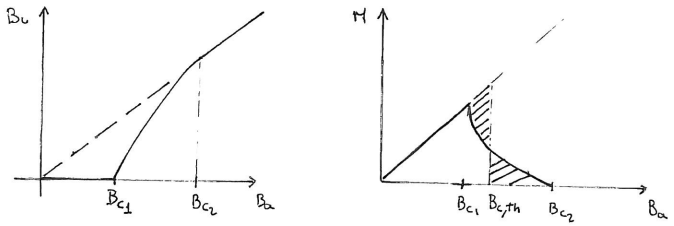
\includegraphics[width=0.7\linewidth]{Immagini - Capitolo 2/SC tipo II.png}
    \caption{andamento in funzione di $B_a$: (i) del campo magnetico interno al superconduttore $\vB_i$; (ii) della magnetizzazione $M$.}
    \label{fig: SC tipo II}
\end{figure}

Il secondo valore critico del campo magnetico $B_{c_2}$ in questo tipo di superconduttori può anche essere cento volte più alto del valore critico $B_c$ nei superconduttori di tipo I, risultando così più utili in applicazioni tecnologiche. I valori di $B_{c_1}$ e $B_{c_2}$ dipendono anch'essi dalla temperatura con un andamento parabolico simile a quello visto in equazione \eqref{eq: valore cricito Bc nei SC di tipo I}. In particolare, nei cristalli perfetti, le linee di flusso sono sistemate in modo regolare secondo il reticolo di Abrikosov, identico a quello osservato nei superfluidi in rotazione. 

\section{Termodinamica dei superconduttori}
La Termodinamica è basata sui principi generali e non dipende dalla descrizione microscopica del modello, essendo quindi in gradi di fornire risultati universali. Si considera il campo magnetico esterno $\vB \equiv \vB_a = \mu_0\vH$ come variabile indipendente e si descrive il sistema utilizzando l'insieme di variabili indipendenti $\{T,p,B\}$, ossia tramite l'energia libera di Gibbs 
\begin{equation}
    G = U - TS +pV - \vm \cdot \vB.
\end{equation}
Poiché $\vm$ e $\vB$ sono paralleli si possono ignorare le proprietà vettoriali e tenere conto solo del segno del momento magnetico. La variazione di energia libera quindi è 
\begin{equation}
    dG = -SdT + Vdp - mdB.
\end{equation}
Si vuole ora confrontare l'energia libera di Gibbs della fase normale con quella della fase superconduttiva.  Questa differenza è intimamente connessa con la natura della transizione di fase. Si supponga che il fattore di demagnetizzazione sia nullo e si trascurino i cambiamenti dovuti alla variazione di pressione. Per il superconduttore, si ha come magnetizzazione $M = m/V = -B/\mu_0$; per cui 
\begin{equation}
    dG_S  = -SdT + \cancelto{0}{Vdp} - mdB = -SdT + \frac{VB}{\mu_0}dB
\end{equation}
ed integrando
\begin{equation}
    G_S(B,T) = G_S(0,T) + \int_0^BdB'\,\frac{VB'}{\mu_0} = G_S(0,T) + \frac{VB^2}{2\mu_0},
\end{equation}
si trova un'espressione dove l'ultimo termine è positivo, indicando che l'energia necessaria per repellere il campo magnetico è positiva. Nel metallo normale, si trascurano le variazioni di energia dovute al campo magnetico poiché le variazioni di magnetizzazione dovute alla superconduttività sono molto più grandi rispetto al paramagnetismo o al diamagnetismo dei conduttori normali, per cui si ha $G_N(B,T) \simeq G_N(0,T)$. In accordo con
\begin{equation}
    G_S(B,T) = G_S(0,T) + \frac{VB^2}{2\mu_0},
\end{equation}
l'energia libera di Gibbs aumenta al crescere del campo magnetico: ad un certo punto necessariamente $G_S(B,T) \ge G_N(B,T)$ e lo stato superconduttore diventa instabile, ritornando allo stato normale. Quindi, deve esistere un valore di soglia $B_c$ tale per cui 
\begin{equation}
    G_S(B_c,T) = G_N(B_c,T) \simeq G_N(0,T) = G_S(0,T) + \frac{VB_c^2}{2\mu_0},
\end{equation}
da cui si ha
\begin{equation}
    G_N(0,T) - G_S(0,T) = \frac{V}{2\mu_0}B_c(T)^2,\quad B_C(T) \simeq B_c(0)\bigg(1 - \frac{T^2}{T_c^2}\bigg),
\end{equation}
dove poiché $G_N(B_c,T_c) = G_S(B_c,T_c)$, allora $B_c(T) \to 0$ per $T \to T_c$, come infatti mostra l'andamento di $B_c(T)$. Dalla differenza di energia libera tra il conduttore normale e il superconduttore, ricordando che $\p G/\p T = -S$, si può determinare la differenza di entropia come
\begin{equation}
    \Delta S= S_N(0,T) - S_S(0,T) = -\frac{VB_c}{\mu_0}\frac{dB_c(T)}{dT} \simeq \frac{2VB_c(0)^2}{\mu_0T_c^2}\bigg(1 - \frac{T^2}{T_c^2}\bigg)T.
\end{equation}
Per $T \to T_c$, la differenza di entropia $\Delta S$ tende ad annullarsi, come accade per il calore latente $\Delta Q = T_c\Delta S$; pertanto, la transizione è del secondo ordine, per $B = 0$. Analogamente, per $T \to 0$, ancora $\Delta Q \to 0$, ossia $\Delta S \to 0$, come ci si aspetta dal terzo principio della Termodinamica. Invece, per $0 < T < T_c$, si ha che
\begin{equation}
    \frac{dB_c(T)}{dT} <0, \quad \Delta S > 0,
\end{equation}
ossia il superconduttore è più ordinato del conduttore normale; dal grafico in figura \ref{fig: S(T) e B(T)} si vede come $S_N$ cresca linearmente con $T$ per basse temperature. Poiché la variazione di energia di Gibbs è
\begin{equation}
    \Delta G(B,T) = G_N(B,T) - G_S(B,T) \simeq G_N(0,T) - G_S(0,T) - \frac{VB^2}{2\mu_0},
\end{equation}
allora la variazione di entropia è
\begin{equation}
    \Delta S(B,T) \simeq \Delta S(0,T) \neq 0,\quad 0 < T < T_c,
\end{equation}
e la transizione di fase, al variare del campo magnetico sulla linea $B = B_c(T)$, è del primo ordine, come mostrato in figura \ref{fig: S(T) e B(T)}.
\begin{figure}[h]
    \centering
    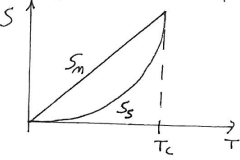
\includegraphics[width=0.4\linewidth]{Immagini - Capitolo 2/S(T).png}
    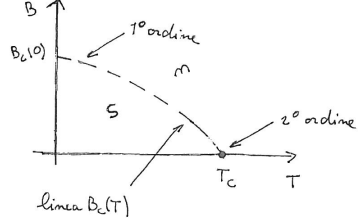
\includegraphics[width=0.4\linewidth]{Immagini - Capitolo 2/B(T).png}
    \caption{andamento in funzione della temperatura: (i) dell'entropia  per le fase normale e di superconduzione; (ii) del campo magnetico.}
    \label{fig: S(T) e B(T)}
\end{figure}

\subsection{Equazioni di London}
L'effetto Meissner-Ochsenfeld è il punto di partenza per la derivazione delle equazioni di London. Si considera un conduttore ideale, quindi, avendo resistenza nulla, le collisioni elettrone-elettrone ed elettrone-reticolo sono nulle. La seconda legge di Newton per il singolo elettrone di massa $m$ è semplicemente $m\va = -e\vE$. Definendo la densità di corrente $\vJ  = -ne\vv$, tale equazione si può riscrivere come
\begin{equation}
    \frac{\p\vJ}{\p t} = \frac{ne^2}{m}\vE.
\end{equation}
Supponendo che quest'ultima sia valida anche per i superconduttori, si trova la prima equazione di London
\begin{equation}
\label{eq: I equazione di London}
    \frac{\p\vJ}{\p t} = \frac{n_Se^2_S}{m_S}\vE,
\end{equation}
dove $n_S = n/2$, $e_S = 2e$ e $m_S = 2m$, dato che in questo regime i portatori di carica sono le coppie di Cooper, come descritto dalla teoria BCS. Diversamente da un conduttore normale, non è la corrente ad essere proporzionale al campo elettrico, ma lo è la sua derivata. Ad ogni modo, la prima equazione di London dà l'impressione che la corrente di un superconduttore possa crescere indefinitamente. In realtà, proprio perché la resistenza è nulla, anche il campo elettrico $\vE$ si annulla nello stato stazionario. Quindi, la variazione temporale di $\vJ$ si annulla, per cui la corrente rimane costante ed è esclusivamente determinata dalla sorgente. 

Si riparte adesso dalla terza equazione di Maxwell $\nabla \times \vE = -\p\vB/\p t$, dalla quale, moltiplicando per $n_Se^2_S/m_S$, si trova
\begin{equation}
    \frac{\p}{\p t}\bigg(\nabla \times \vJ_S + \frac{n_Se_S^2}{m_S}\vB\bigg) = 0.
\end{equation}
All'interno di un conduttore ideale, il flusso attraverso un circuito arbitrario non può variare nel tempo. Tuttavia, per un superconduttore, il campo magnetico all'interno non solo è costante, ma è proprio nullo. Da questo si trova la seconda equazione di London
\begin{equation}
\label{eq: II equazione di London}
    \nabla \times \vJ_S + \frac{n_Se_S^2}{m_S}\vB = 0.
\end{equation}
Dalla relazione $\vB = \nabla \times \vA$ si ha 
\begin{equation}
    \nabla \times \bigg(\vJ_S + \frac{n_Se_S^2}{m_S}\vA\bigg) = 0,
\end{equation}
da cui si trova immediatamente, imponendo il gauge di London $\nabla \cdot \vA = 0$, la forma della densità di corrente 
\begin{equation}
    \vJ_S = -\frac{n_Se_S^2}{m_S}\vA.
\end{equation}
Di conseguenza, dall'equazione di Maxwell per il potenziale vettore
\begin{equation}
    \square\vA = \nabla^2\vA - \cancelto{0}{\frac{1}{c^2}\frac{\p^2\vA}{\p t^2}} = -\mu_0\vJ_s = \frac{\mu_0n_Se_S^2}{m_S}\vA
\end{equation}
si trova l'equazione di Klein-Gordon per tale campo
\begin{equation}
    \bigg(\nabla^2 - \frac{c^2m_\gamma^2}{\hbar^2}\bigg)\vA = 0,\quad m_\gamma \equiv \sqrt{\frac{\mu_0n_Se_S^2}{m_S}}\frac{\hbar}{c}.
\end{equation}
Da questo risultato si conclude che in un superconduttore dove si verifica l'effetto di Meissner-Ochsenfeld corrisponde all'acquisizione da parte dei fotoni al suo interno di una massa pari a $m_\gamma$, in analogia con il meccanismo di Higgs-Anderson in Teoria dei campi. 

Una delle applicazioni più importanti della seconda equazione di London è la descrizione dello schermaggio nei superconduttori nello stato di Meissner. Fino ad ora si è sostenuto che il campo magnetico fosse completamente espulso in tale stato; tuttavia, se ciò fosse vero, una corrente di densità infinita dovrebbe circolare sulla superficie del superconduttore. Per discutere questo fenomeno, si assume che il superconduttore occupi lo spazio per $x > 0$ e che il campo magnetico sia $\vB = (0,0,B_{0z})$, come mostrato in figura \ref{fig: lunghezza di penetrazione}.
\begin{figure}[h]
    \centering
    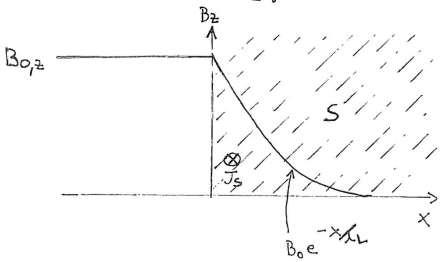
\includegraphics[width=0.5\linewidth]{Immagini - Capitolo 2/lunghezza di penetrazione.png}
    \caption{andamento del campo magnetico $\vB$ in un superconduttore.}
    \label{fig: lunghezza di penetrazione}
\end{figure}
Se si inserisce la seconda equazione di London nella quarta equazione di Maxwell $\nabla \times \vB = \mu_0\vJ_S$ si ha
\begin{equation}
    \nabla \times \nabla \times \vB + \frac{\mu_0n_Se_S^2}{m_S}\vB = 0,
\end{equation}
da cui, poiché $\nabla \times \nabla \times \vf = \nabla(\nabla \cdot \vf) - \nabla^2\vf$ e $\nabla \cdot \vB = 0$, si trova
\begin{equation}
    \begin{split}
        \nabla^2\vB - \frac{\mu_0n_Se_S^2}{m_S}\vB = \frac{d^2B_z(x)}{dx^2} - \frac{B_z(x)}{\Lambda_L^2} = 0,\quad \Lambda_L = \sqrt{\frac{m_s}{\mu_0n_Se_S^2}},
    \end{split}
\end{equation}
dove $\Lambda_L$ è la lunghezza di penetrazione di London, la quale è legata alla massa acquisita dal fotone da $\Lambda_L = \hbar/cm_\gamma$. La soluzione dell'equazione in $B_z(x)$ è
\begin{equation}
    B_z(x) = B_{0z}e^{-x/\Lambda_L},
\end{equation}
che inserita nella quarta equazione di Maxwell restituisce la variazione spaziale della corrente di screening
\begin{equation}
    J_{S,y}(x) = J_{0y}e^{-x/\Lambda_L} = \frac{B_{0z}}{\mu_0\Lambda_L}e^{-x/\Lambda_L}.
\end{equation}
Quindi, sia il campo magnetico che la densità di corrente decrescono esponenzialmente all'interno di un superconduttore con una lunghezza di penetrazione $\Lambda_L$ data dall'inverso della massa acquisita dal fotone in tale mezzo. Inoltre, il campo magnetico applicato e la corrente sono proporzionali, $B_{0z} = \mu_0\Lambda_LJ_{0y}$.

\section{Modello di Landau-Ginzburg}
La teoria di Landau-Ginzburg per la superconduttività è stata formulata utilizzando un approccio generale alle transizioni di fase del secondo ordine. Tale teoria è caratterizzata da un parametro d'ordine il cui valore all'equilibrio è nullo nella fase disordinata a $T \ge T_c$ ma diventa diverso da zero per $T < T_c$. In particolare, per la superconduttività, la teoria di Landau-Ginzburg postula l'esistenza di un parametro d'ordine $\psi$, il quale caratterizza lo stato superconduttore nello stesso modo in cui la magnetizzazione caratterizza lo stato di un ferromagnete. Si assume quindi che all'equilibrio
\begin{equation} 
    \begin{cases}
        \psi = 0, \quad T \ge T_c \\
        \psi \neq 0, \quad T \le T_c
    \end{cases},\quad \psi \equiv \psi_0(T).
\end{equation}
Il parametro d'ordine è postulato essere complesso, facendo riferimento ad una funzione d'onda macroscopica per il superconduttore analoga a quella dell'elio-II. Inizialmente, il significato di $\psi$ non era chiaro, ma con lo sviluppo della teoria BCS si intuì fosse legato alla densità di coppie di Cooper. Si assume che l'energia libera del superconduttore dipenda in modo ``smooth'' dal parametro d'ordine. Inoltre, poiché $\psi$ è complesso, l'energia libera deve dipendere solo da $\psi^*\psi = |\psi|^2$, per cui
\begin{equation}
   \Delta f \equiv f_S(T) - f_N(T) = a(T)|\psi|^2 + \frac{b(T)}{2}|\psi|^4 + o(|\psi|^6),
\end{equation}
dove $f = F/V$ è l'energia libera di Helmoltz e $f_S$ ed $f_n$ sono quelle relative allo stato superconduttivo e normale, rispettivamente, mentre i parametri $a(T)$ e $b(T)$ sono parametri fenomenologici che dipendono in modo ``smooth'' dalla temperatura $T$. Se si grafica l'andamento di $\Delta f$ in funzione di $|\psi|$, mostrato in figura \ref{fig: energia di Helmoltz (teoria L-G)}, si presentano due casi:
\begin{enumerate}
    \item se $a(T) > 0$, la curva ha un minimo in $|\psi|^2 = |\psi_0|^2 = 0$ e $f_S > f_N$;
    \item se $a(T) < 0$, la curva ha un minimo in $|\psi|^2 = |\psi_0|^2 = -a(T)/b(T)$.
\end{enumerate}
Nel modello di Landau-Ginzburg si assume che 
\begin{equation}
    \begin{cases}
        a(T) > 0,\quad T > T_c \\
        a(T) = 0,\quad T = T_c \\
        a(T) < 0,\quad T < T_c
    \end{cases}
\end{equation}
e che $b(T)$ vari lentamente attorno a $T = T_c$, per cui 
\begin{equation}
    \begin{cases}
        a(T) \simeq \tilde{a}(T - T_c) \\
        b(T) \simeq b
    \end{cases},
\end{equation}
mentre
\begin{equation}
    |\psi_0| = \begin{cases}
        0,\quad T \ge T_c \\
        \bigg(\dfrac{\tilde{a}}{b}\bigg)^{1/2}(T - T_c)^{1/2},\quad T < T_c
    \end{cases},
\end{equation}
dove $|\psi_0|$ minimizza $\Delta f \equiv f_S - f_N$.
\begin{figure}[h]
    \centering
    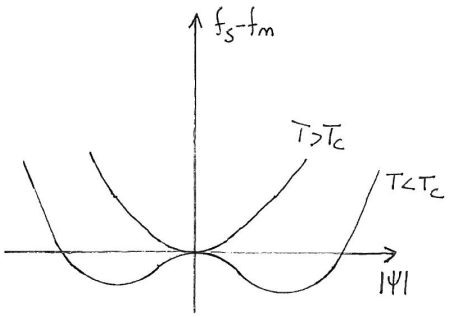
\includegraphics[width=0.4\linewidth]{Immagini - Capitolo 2/energia di Helmoltz (teoria L-G).png}
    \caption{andamento di $\Delta f \equiv f_S - f_N$ in funzione di $|\psi|$.}
    \label{fig: energia di Helmoltz (teoria L-G)}
\end{figure}
Sostituendo $|\psi|^2 = |\psi_0|^2 = \tilde{a}(T_c - T)/b$, si ha
\begin{equation}
    \begin{split}
        f_S(T) - f_N(T) &= \tilde{a}(T - T_c)\bigg(\frac{\tilde{a}}{b}\bigg)(T_c - T) + \frac{b}{2}\bigg(\frac{\tilde{a}}{b}\bigg)^2(T_c - T)^2 \\
        &= -\frac{\tilde{a}^2}{2b}(T - T_c)^2.
    \end{split}
\end{equation}
Poiché, la differenza di energia libera di Gibbs è
\begin{equation}
    G_N(0,T) - G_S(0,T) = \frac{\mu_0H_c^2V}{2} = F_N(0,T) - F_S(0,T) + \mu_0 \cancelto{0}{(\vH \cdot \vM)},
\end{equation}
si ha
\begin{equation}
    F_S(0,T) - F_N(0,T) = -\frac{\mu_0VH_c^2}{2},
\end{equation}
che confrontata con $\Delta f(0,T) = -\tilde{a}^2(T - T_c)^2/2b$, restituisce
\begin{equation}
    H_c = \frac{\tilde{a}(T_c - T)}{\sqrt{\mu_0 b}},
\end{equation}
che coincide con l'approssimazione lineare a $T \simeq T_c$ di 
\begin{equation}
    H_c(T) = H_c(0)\bigg(1 - \frac{T^2}{T_c^2}\bigg) = \frac{H_c(0)}{T_c^2}(T_c - T)(T_c + T) \simeq \frac{2H_c(0)}{T_c}(T_c - T).
\end{equation}

\subsection{Sistemi non omogenei}
Per completare la teoria di Landau-Ginzburg per la superconduttività, si permette al parametro d'ordine $\psi$ di dipendere anche dalle coordinate spaziali $\vr$. La teoria in questo modo comincia ad assomigliare alla teoria dei superfluidi 
\begin{equation}
    f_S(T,\vr) - f_N(T,\vr) = \frac{\hbar^2}{2m^*}|\nabla\psi(\vr)|^2 + a(T)|\psi(\vr)|^2 + \frac{b(T)}{2}|\psi(\vr)|^4,
\end{equation}
dove si nota come ponendo $\psi(\vr) = \psi$ si ritorni al caso precedente. Inoltre, il parametro $m^*$, avente le dimensioni di una massa, determina il costo di energia associato a gradienti non nulli di $\psi(\vr)$. Quindi, $m^*$ gioca il ruolo di massa efficace nel sistema quantistico con funzione d'onda macroscopica $\psi(\vr)$. L'energia totale del sistema è
\begin{equation}
    F_S(T) = F_N(T) + \int_Vd^3r\,\bigg[-\frac{\hbar^2}{2m^*}\psi^*\nabla^2\psi + a(T)\psi^*\psi + \frac{b}{2}(\psi^*\psi)^2\bigg]
\end{equation}
La configurazione di equilibrio termodinamico si ha imponendo
\begin{equation}
    \frac{\delta F_S}{\delta \psi^*} = 0,
\end{equation}
ossia richiedendo che la funzione integranda sia minima; da qui si ottiene
\begin{equation}
    \bigg[-\frac{\hbar^2}{2m^*}\nabla^2 + a + b|\psi(\vr)|^2\bigg]\psi(\vr) = 0,
\end{equation}
che coincide all'equazione stazionaria di Gross-Pitaevskii per i gasi diluiti a bassa temperatura.

\subsection{Interfaccia nei superconduttori}
L'equazione non lineare di Schr\"odinger ha svariate applicazioni, ad esempio può essere usata per studiare la risposta del parametro d'ordine ad una perturbazione esterna. Si consideri un modello semplice di interfaccia tra un superconduttore ed un conduttore normale, come mostrato in figura \ref{fig: interfaccia SC I}; l'equazione da risolvere è
\begin{equation}
    -\frac{\hbar^2}{2m^*}\frac{d^2\psi(x)}{dx^2} + a(T)\psi(x) + b\psi(x)^3 = 0,
\end{equation}
con le condizioni al contorno
\begin{equation}
    \begin{cases}
        \psi(x) \neq 0,\quad x > 0 \\
        \psi(x) = 0,\quad x < 0
    \end{cases}.
\end{equation}
\begin{figure}[h]
    \centering
    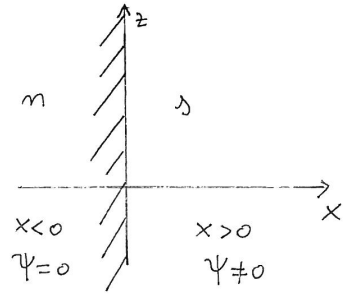
\includegraphics[width=0.35\linewidth]{Immagini - Capitolo 2/interfaccia SC I.png}
    \caption{interfaccia tra un superconduttore ed un conduttore normale.}
    \label{fig: interfaccia SC I}
\end{figure}

Ricordando l'equazione soddisfatta da $f(z) = \tanh{z}$,
\begin{equation}
    \frac{df(z)}{dz} = 1 - f(z)^2,
\end{equation}
da cui si può calcolare
\begin{equation}
    \begin{split}
        \frac{d^2f(z)}{dz^2} = -2f(z)[1 - f(z)^2] = -2f(x) + 2f(z)^3,
    \end{split}
\end{equation}
si trova un'equazione con la medesima forma di quella che si intende risolvere
\begin{equation}
    -\frac{d^2f(z)}{dz^2} - 2f(x) + 2f(z)^3 = 0.
\end{equation}
Usando infatti l'ansatz $\psi(x) = \alpha\phi(x\beta)$, e usando il fatto che $a(T) = -|a(T)|$, si ha
\begin{equation}
    \begin{split}
        -\frac{\hbar^2\beta^2\alpha}{2m^*}\frac{d^2\phi(x\beta)}{d(x\beta)^2} - |a(T)|\alpha\phi(x\beta) + \alpha^3b\phi(x\beta)^3 &= 0 \\
        -\frac{d^2\phi(x\beta)}{d(x\beta)^2} - \frac{|a(T)|}{\bigg(\dfrac{\hbar^2\beta^2}{2m^*}\bigg)}\phi(x\beta) + \frac{\alpha^2b}{\bigg(\dfrac{\hbar^2\beta^2}{2m^*}\bigg)}\phi(x\beta)^3 &= 0,
    \end{split}
\end{equation}
Quindi, definendo i parametri $\alpha$ e $\beta$ in modo opportuno imponendo
\begin{equation}
    \begin{cases}
        \dfrac{|a(T)|}{\bigg(\dfrac{\hbar^2\beta^2}{2m^*}\bigg)} = 2 \\[5ex]
        \dfrac{\alpha^2b}{\bigg(\dfrac{\hbar^2\beta^2}{2m^*}\bigg)} = 2
    \end{cases}\quad\Longrightarrow\quad
    \begin{cases}
        \alpha = \sqrt{\dfrac{|a(T)|}{b}} \\[2ex]
        \beta = \sqrt{\dfrac{|a(T)|m^*}{\hbar^2}}
    \end{cases},
\end{equation}
si trova la soluzione 
\begin{equation}
    \psi(x) = \sqrt{\frac{|a(T)|}{b}}\phi\bigg(x\sqrt{\frac{|a(T)|m^*}{\hbar^2}}\bigg) \equiv \psi_0\tanh{\bigg[\frac{x}{\sqrt{2}\xi(T)}\bigg]},
\end{equation}
dove si è definita la lunghezza di healing, o di coerenza, come 
\begin{equation}
    \xi(T) \equiv \frac{\hbar}{\sqrt{2m^*|a(T)|}} = \frac{\hbar}{\sqrt{2m^*\tilde{a}(T - T_c)}},
\end{equation}
che racchiude l'informazione di quanto la funzione d'onda cambi all'interfaccia rispetto allo stato lontano da essa, che tende a $\psi_0$, come mostrato in figura \ref{fig: parametro d'ordine SC in x}. Il fatto che $\xi(T) \propto |T - T_c|^{-1/2}$ implica che la lunghezza di healing diverge alla temperatura critica con un esponente critico pari a $-1/2$. Da questo risultato è possibile ottenere l'energia associata alla penetrazione dell'interfaccia all'interno del superconduttore in $x > 0$; in altre parole, si vuole determinare la differenza in energia tra le due configurazioni mostrate in figura \ref{fig: interfaccia SC II}. L'energia libera di bulk nel volume $V = \Sigma x_0$ è 
\begin{equation}
    F_S(0,T) - F_N(0,T) = -\mu_0\frac{VH_c^2}{2} = -\frac{a^2}{2b}\Sigma x_0,
\end{equation}
a cui corrisponde un'energia per unità di superficie 
\begin{equation}
    \sigma_{bulk} = \frac{F_S(0,T) - F_N(0,T)}{S} = -\int_0^{x_0}dx\,\frac{\mu_0H_c^2}{2}
\end{equation}
e una differenza di energia pari a 
\begin{equation}
    \begin{split}
        \sigma &= \sigma_\psi - \sigma_{bulk} \\
        &= \int_0^\infty dx\,\bigg[\frac{\hbar^2}{2m^*}\bigg(\frac{d\psi(x)}{dx}\bigg)^2 + a(T)\psi(x)^2 + \frac{b}{2}\psi(x)^4 + \frac{\mu_0H_c^2}{2}\bigg].
    \end{split}
\end{equation}
Quest'ultima, dal calcolo dovuto a de Gennes, risulta essere pari a
\begin{equation}
    \sigma \simeq (1.89)\times\frac{1}{2}\mu_0H_c^2\xi(T).
\end{equation}
\begin{figure}[h]
    \centering
    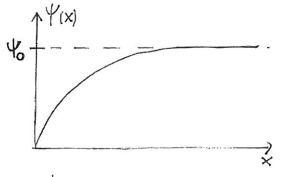
\includegraphics[width=0.4\linewidth]{Immagini - Capitolo 2/parametro d'ordine SC in x.png}
    \caption{andamento del parametro d'ordine $\psi$ in funzione di $x$.}
    \label{fig: parametro d'ordine SC in x}
\end{figure}
\begin{figure}[h]
    \centering
    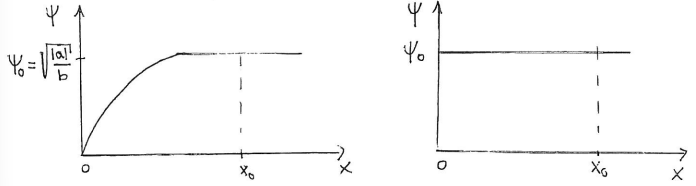
\includegraphics[width=0.9\linewidth]{Immagini - Capitolo 2/interfaccia SC II.png}
    \caption{configurazioni dove $\psi(x)$ è: (i) pari a $\sqrt{|a(T)|/b}$; (ii) costante.}
    \label{fig: interfaccia SC II}
\end{figure}

\subsection{Teoria di Landau-Ginzburg in campo magnetico}
La vera potenzialità dell'approccio di Landau e Ginzburg applicato ai superconduttori diventa evidente solo quando si inserisce il contributo del campo magnetico. Infatti, fino ad ora quanto discusso non include gli effetti legati alla caratteristica del superfluido di non essere neutro, ma carico, essendo appunto una supercorrente. L'introduzione del contributo di campo magnetico viene postulato da Landau e Ginzburg assumendo un accoppiamento minimo tra il parametro d'ordine $\psi(\vr)$ e $\vB$, ottenuto dalla sostituzione
\begin{equation}
    -i\hbar\nabla \to -i\hbar\nabla - q\vA,
\end{equation}
equivalente a considerare $\psi(\vr)$ come una funzione d'onda di particelle cariche con carica $q$. In particolare, risultava che per i tutti i superconduttori la carica era $q = 2e \equiv e_S$, per cui
\begin{equation}
    -i\hbar\nabla \to -i\hbar\nabla - 2e\vA.
\end{equation}
Di nuovo, la spiegazione di questo avvenne con lo sviluppo della teoria BCS e con la comprensione del legame tra tale teoria e quella di Landau-Ginzburg. Ad ogni modo, ora l'energia libera nella teoria di Landau-Ginzburg è
\begin{equation}
    f_S(T) - f_N(T) = \frac{1}{2m^*}|(-i\hbar\nabla - 2e\vA)\psi(\vr)|^2 + a(T)|\psi(\vr)|^2 + \frac{b}{2}|\psi(\vr)|^4.
\end{equation}
Quest'ultima espressione contiene l'accoppiamento tra la funzione d'onda del condensato e il campo magnetico attraverso il potenziale vettore $\vA$, con $\vB = \nabla \times \vA$. Tuttavia, a questo punto non è possibile separare completamente il condensato dal campo magnetico e nel calcolo dell'energia libera bisogna pertanto includere anche il termine 
\begin{equation}
    \Delta F_{\vB} = \frac{1}{2\mu_0}\int_{\R^3} d^3r\,\vB(\vr)^2,
\end{equation}
dove l'integrale in $\R^3$ è inteso su tutto lo spazio. Quindi, così facendo si ottiene che $\Delta F \equiv F_S(T) - F_N(T)$ è data da
\begin{equation}
    \begin{split}
        \Delta F &= \int_V d^3r\,\bigg[\frac{1}{2m^*}|(-i\hbar\nabla - 2e\vA)\psi(\vr)|^2 + a(T)|\psi(\vr)|^2 + \frac{b}{2}|\psi(\vr)|^4\bigg] \\
        &+ \frac{1}{2\mu_0}\int_{\R^3} d^3r\,\vB(\vr)^2.
    \end{split}
\end{equation}
Quindi, $\Delta F$ è costituita da tre contributi $\Delta F = \Delta F_\psi + \Delta F_{\vB} + \Delta F_{int}$, dove 
\begin{align}
    \Delta F_\psi &= \int_V d^3r\,\bigg[\frac{\hbar^2}{2m}|\nabla^2\psi| + a(T)|\psi(\vr)|^2 + \frac{b}{2}|\psi(\vr)|^4\bigg], \\
    \Delta F_{\vB} &= \frac{1}{2\mu_0}\int_{\R^3} d^3r\,\vB(\vr)^2, \\
    \begin{split}
        \Delta F_{int} &= \int_V\frac{d^3r}{2m^*}[-2ei\hbar\nabla\psi^*(\vr)\vA\psi(\vr) + 2ei\hbar\nabla\psi(\vr)(\vA\psi(\vr))^* \\
        &+ (2e)^2|\psi(\vr)|^2(\vA \cdot \vA)] \\
        &= \int_V d^3r\,\bigg[\frac{2ei\hbar}{2m^*}(\psi^*\nabla\psi - \psi\nabla\psi^*)\cdot\vA + \frac{(2e)^2}{2m^*}|\psi|^2(\vA\cdot\vA)\bigg].
    \end{split}
\end{align}
In particolare, l'energia di interazione può essere sempre scritta come
\begin{equation}
    F_{int} = -\int_Vd^3r\,\vJ_S\cdot\vA,
\end{equation}
ovvero
\begin{equation}
    \frac{\delta F_{int}}{\delta \vA} = -\vJ_S,
\end{equation}
per cui la densità di supercorrente è
\begin{equation}
    \vJ_S = -\frac{2ei\hbar}{2m^*}(\psi^*\nabla\psi - \psi\nabla\psi^*) - \frac{(2e)^2}{m^*}|\psi|^2\vA.
\end{equation}
Inoltre, ponendo $\psi(\vr) = |\psi(\vr)|e^{i\theta}$, il termine $\psi^*\nabla\psi - \psi\nabla\psi^* = 2i|\psi(\vr)|\nabla\theta$, quindi si può scrivere $\vJ_S$ come
\begin{equation}
    \begin{split}
        \vJ_S &= \frac{2e\hbar}{m^*}|\psi(\vr)|^2\nabla\theta - \frac{(2e)^2}{m^*}|\psi(\vr)|^2\vA \\
        &= \frac{(2e)^2}{m^*}|\psi(\vr)|^2\bigg(\frac{\hbar}{2e}\nabla\theta - \vA\bigg).
    \end{split}
\end{equation}
Il parametro d'ordine $\psi(\vr)$ è soluzione dell'equazione di Gross-Pitaesvkii con accoppiamento minimale
\begin{equation}
    -\frac{\hbar^2}{2m^*}\bigg(\nabla - \frac{2ei}{\hbar}\vA\bigg)^2 + [a(T) + b|\psi(\vr)|^2]\psi(\vr) = 0.
\end{equation}

\subsection{Simmetria di gauge}
Il parametro d'ordine dei superconduttori $\psi(\vr) = |\psi(\vr)|e^{i\theta(\vr)}$ ha un'ampiezza ed una fase. Da questo punto di vista la situazione è molto simile a quella dei superfluidi, ma con una differenza sostanziale. Per capire di cosa si tratta si consideri l'operatore momento 
\begin{equation}
    \hatp = -i\hbar\nabla - 2e\vA,
\end{equation}
se si trasforma $\psi(\vr)$ con un fattore di fase moltiplicativo $\psi(\vr) \to \psi(\vr)e^{i\chi(\vr)}$ si ha 
\begin{equation}
    \begin{split}
        \hatp\psi(\vr)e^{i\chi(\vr)} &= e^{i\chi(\vr)}(-i\hbar\nabla - 2e\vA)\psi(\vr) + \hbar\psi(\vr)e^{i\chi(\vr)}\nabla\chi(\vr) \\
        &= e^{i\chi(\vr)}\bigg[-i\hbar\nabla - 2e\bigg(\vA - \frac{\hbar}{2e}\nabla\chi(\vr)\bigg)\bigg]\psi(\vr),
    \end{split}
\end{equation}
da cui si può dedurre che, se si operano simultaneamente le trasformazioni di gauge
\begin{equation}
\label{eq: trasformazione di gauge locale superconduttori}
    \begin{cases}
        \psi(\vr) \to \psi(\vr)e^{i\chi(\vr)} \\[2ex]
        \vA(\vr) \to \vA(\vr) + \dfrac{\hbar}{2e}\nabla\chi(\vr)
    \end{cases},
\end{equation}
la teoria presenta un'invarianza di gauge locale; infatti, sia la fase della funzione d'onda $e^{i\chi(\vr)}$ che il potenziale vettore $\vA$ dipendono dalla scelta del gauge, ma tutte le osservabili sono invarianti. Ora si consideri la corrente
\begin{equation}
    \vJ_S = \frac{(2e)^2}{m^*}|\psi(\vr)|^2\bigg(\frac{\hbar}{2e}\nabla\theta - \vA\bigg),
\end{equation}
che è come ci si aspetta invariante per la trasformazione di gauge locale \eqref{eq: trasformazione di gauge locale superconduttori}, e se ne calcoli il rotore
\begin{equation}
    \nabla \times \vJ_S = 0 - \frac{(2e)^2}{m^*}|\psi_0|^2(\nabla \times \vA) = -\frac{(2e)^2}{m^*}|\psi_0|^2\vB,
\end{equation}
dove si è assunto che $|\psi|^2 = |\psi_0|^2 = costante$ e si è usata la proprietà $\nabla \times (\nabla\vf) = 0$ per ogni $\vf$. Si nota che tale rotore coincide con la seconda equazione di London \eqref{eq: II equazione di London}, a patto di identificare
\begin{equation}
    m_S = m^* = 2m_e,\quad e_S = 2e,\quad n_S = |\psi_0|^2.
\end{equation}
Quindi, poiché la seconda equazione di London è equivalente all'effetto di Meissner-Ochesenfeld, si è così verificato che il modello di Landau e Ginzburg descrive la fisica dei superconduttori. Inoltre, considerando il regime stazionario dove si ha $\p_t\vE = 0$ e assumendo l'assenza di correnti esterne, si ha che
\begin{equation}
    \nabla \times \vB = \mu_0\vJ_s\quad \Longrightarrow\quad \nabla \times \nabla \times \vB = \mu_0(\nabla \times \vJ_s),
\end{equation}
per cui 
\begin{equation}
    \nabla^2\vB = -\frac{(2e)^2\mu_0}{m^*}|\psi_0|^2\vB = -\frac{c^2m_\gamma^2}{\hbar^2}\vB,
\end{equation}
che riarrangiata corrisponde all'equazione
\begin{equation}
    \nabla^2\vB + \frac{c^2m_\gamma^2}{\hbar^2}\vB = 0,\quad m_\gamma = \frac{\hbar}{c}\sqrt{\frac{\mu_0(2e)^2|\psi_0|^2}{m}}.
\end{equation}
Dunque, la massa acquisita dal fotone tramite il meccanismo di Anderson-Higgs è proporzionale al modulo del parametro d'ordine all'equilibrio. L'acquisizione di massa da parte del fotone in particolare deriva dalla variazione di fase della funzione d'onda, questo cambiamento longitudinale può essere assorbito da $\vA$: nel vuoto il campo è ortogonale alla direzione di propagazione, ma adesso il campo acquisisce un grado di libertà longitudinale, passando da due a tre gradi di libertà, permettendogli appunto di acquisire massa.
\begin{obs}
    Si può seguire un procedimento analogo per il potenziale vettore $\vA$ nel caso omogeneo con $\theta = costante$ ponendosi nel gauge di London con $\nabla \cdot \vA = 0$.
\end{obs}

\section{Quantizzazione del flusso magnetico}
In generale, la fase $\theta(\vr)$ della funzione d'onda macroscopica nei superconduttori è ben definita a meno di multipli di $2\pi$. La differenza $\Delta\theta$ tra due punti del superconduttore si ottiene calcolando l'integrale di linea sulla curva $L$ che unisce i due punti 
\begin{equation}
    \Delta\theta = \oint_L\nabla\theta \cdot d\vl = 2\pi n,\quad n \in \Z.
\end{equation}
Per dimostrare la quantizzazione del flusso di campo magnetico, si consideri un superconduttore a forma toroidale, quindi un dominio connesso, ma non semplicemente. Immergendo il toroide in un campo magnetico esterno, che passa attraverso il foro, mentre all'esterno viene deviato. L'esistenza di una funzione d'onda macroscopica ha una conseguenza importante per il flusso del flusso di campo magnetico all'interno del foro. Si consideri ora di nuovo l'espressione della corrente
\begin{equation}
    \vJ_S = \frac{(2e)^2}{m^*}|\psi|^2\bigg(\frac{\hbar}{2e}\nabla\theta - \vA\bigg),
\end{equation}
integrandola su un cammino chiuso all'interno del superconduttore dove $\vJ_S = \vo$, assumendo $|\psi|^2 = |\psi_0|^2 = costante$, si ha
\begin{equation}
    \oint_L\bigg(\vA - \frac{h}{2e}\nabla\theta\bigg)\cdot d\vl = 0,
\end{equation}
da cui, calcolando gli integrali dei due termini separatamente, si hanno
\begin{equation}
    \frac{\hbar}{2e}\oint_L\nabla\theta\cdot d\vl = \dfrac{nh}{2e},\quad n \in \Z
\end{equation}
e
\begin{equation}
    \oint_L \vA \cdot d\vl = \int_\Sigma(\nabla \times \vA)\cdot d\bm{\Sigma} = \int_\Sigma\vB \cdot \bm{\Sigma} = \Phi.
\end{equation}
Dunque, il flusso di campo magnetico all'interno del foro è un multiplo intero di un quanto di flusso $\Phi_0$, chiamato spesso ``flussone'', dato da
\begin{equation}
    \Phi_0 = \frac{h}{2e} \simeq \SI{2.05e-15}{\tesla\meter\squared},
\end{equation}

\subsection{Effetto Josephson}
La previsione teorica di Josephson consisteva tra due materiali superconduttori separati da una piccola barriera di isolante si instaura una corrente spontanea $I_S = I_C\sin{(\Delta\theta_0)}$, dove $\Delta\theta_0$ è la differenza di fase tra le due funzioni d'onda.

Inizialmente, quello che si cerca di capire una volta ipotizzato che ai superconduttori può essere associata una funzione d'onda macroscopica e complessa, è cercare la prova dell'esistenza o meno di una fase. L'effetto Josephson può essere indotto riducendo lo spessore dello strato isolante tra due superconduttori a circa $\SI{10}{\angstrom}$, si ottiene una sovrapposizione non nulla delle funzioni d'onda macroscopiche e si instaura la corrente di superconduzione, oppure al contrario instaurando una differenza di potenziale tra i due materiali, che a sua volta genera una supercorrente alternata con frequenza $\omega = 2e\Delta V/\hbar$. L'apparato sperimentale consiste nel porre a contatto due cavi superconduttori, tra i quali si deposita uno strato di ossido molto sottile, così che le funzioni d'onda si sovrappongano nelle vicinanze di questa giunzione isolante, chiamata giunzione di Josephson. Si preparano quindi due superconduttori inizialmente separati e si abbassa la temperatura sotto la soglia critica, cosicché la funzione d'onda acquisisca un valore di aspettazione non nullo nello stato fondamentale. 

Si considera ora l'equazione di Schr\"odinger per due superconduttori accoppiati da un termine di interazione 
\begin{equation}
\label{eq: equazioni superconduttori giunzione di Josephson}
    \begin{cases}
        i\hbar\dfrac{\p \psi_1}{\p t} = \mu_1\psi_1 + k\psi_2 \\[2ex]
        i\hbar\dfrac{\p \psi_2}{\p t} = \mu_2\psi_2 + k\psi_1
    \end{cases},
\end{equation}
dove $\mu_1$ e $\mu_2$ rappresentano i potenziali chimici dei due superconduttori, mentre la costante $k$ riflette l'intensità dell'accoppiamento. In assenza della giunzione, le due funzioni d'onda sono descritte dalle leggi 
\begin{equation}
    \psi_i(t) = \psi_{0,i}e^{-i\mu_it/\hbar},\quad i = \{1,2\}.
\end{equation}
Nel caso di una differenza di potenziale alla giunzione nulla, i potenziali chimici sono identici $\mu_1 = \mu_2 \equiv \mu$, invece una differenza di potenziale $\Delta V \neq 0$ sposta i livelli di Fermi dei due superconduttori in modo che $\mu_2 - \mu_1 = -2e\Delta V$. Inoltre, per semplificare la trattazione, si assume che i due superconduttori siano dello stesso materiale e abbiano la medesima densità di portatori di supercorrente, $n_{S_1} = n_{S_2} \equiv n_S$. Quindi, se si inserisce $\psi_i(t) = \sqrt{n_{S_i}(t)}\exp{[i\theta_i(t)]}$, nelle equazioni accoppiate \eqref{eq: equazioni superconduttori giunzione di Josephson} si hanno
\begin{equation}
    \begin{cases}
        i\hbar\dfrac{\p}{\p t}[\sqrt{n_{S_1}}(t)]e^{i\theta_1(t)} - \hbar\dot{\theta}_1\sqrt{n_S}e^{i\theta_1} = \mu_1\sqrt{n_S}e^{i\theta_1} + k\sqrt{n_S}e^{i\theta_2} \\[2ex]
        i\hbar\dfrac{\p}{\p t}[\sqrt{n_{S_2}}(t)]e^{i\theta_2(t)} - \hbar\dot{\theta}_2\sqrt{n_S}e^{i\theta_2} = \mu_2\sqrt{n_S}e^{i\theta_2} + k\sqrt{n_S}e^{i\theta_1}
    \end{cases}
\end{equation}
che si possono riscrivere come
\begin{equation}
    \begin{cases}
        \dfrac{i\hbar}{2}\dot{n}_{S_1} - \hbar\dot{\theta}_1n_S = \mu_1 n_S + kn_Se^{i(\theta_2 - \theta_1)} \\[2ex]
        \dfrac{i\hbar}{2}\dot{n}_{S_2} - \hbar\dot{\theta}_2n_S = \mu_2 n_S + kn_Se^{i(\theta_1 - \theta_2)}
    \end{cases},
\end{equation}
separando poi la parte reale da quella immaginaria rispettivamente 
\begin{equation}
    \Re :
    \begin{cases}
        \dot{\theta}_1 = -\dfrac{\mu_1}{\hbar} - \dfrac{k}{\hbar}\cos{(\theta_2 - \theta_1)} \\[2ex]
        \dot{\theta}_2 = -\dfrac{\mu_2}{\hbar} - \dfrac{k}{\hbar}\cos{(\theta_2 - \theta_1)}
    \end{cases},\quad \Im :
    \begin{cases}
        \dot{n}_{S_1} = \dfrac{2k}{\hbar}n_S\sin{(\theta_2 - \theta_1)} \\[2ex]
        \dot{n}_{S_2} = -\dot{n}_{S_1}
    \end{cases}
\end{equation}
e combinandole, si ottengono le equazioni
\begin{equation}
\label{eq: equazioni effetto Josephson}
    \begin{cases}
        \dot{n}_{S_1} = \dfrac{2k}{\hbar}\sin{(\theta_2 - \theta_1)} = -\dot{n}_{S_2} \\[2ex]
        \hbar(\dot{\theta}_2 - \dot{\theta}_1) = -(\mu_2 - \mu_1) = 2e\Delta V
    \end{cases}.
\end{equation}
Si considera come primo caso quello in cui la differenza di potenziale alla giunzione è nulla. Se $\Delta V = 0$, allora la differenza di fase è indipendente dal tempo, per cui anche $\dot{n}_S$ è costante e nella giunzione si instaura una supercorrente continua. Essendo tale corrente proporzionale a sua volta a $\dot{n}_{S_1}$ si può scrivere
    \begin{equation}
        I_S = I_C\sin{(\theta_2 - \theta_1)}.
    \end{equation}
Questo fenomeno, ossia lo scorrere di una corrente attraverso un contatto isolante senza generare una differenza di potenziale prende il nome di ``effetto Josephson in DC''. Negli esperimenti si opera tipicamente al contrario imponendo una corrente $I_S$ attraverso la giunzione e poi misurando $\Delta V$, dove $\Delta V = 0$ per $I_S < I_C$, mentre $\Delta V \neq 0$ per $I_S > I_C$. In particolare, la corrente critica $I_C$ dipende dalla densità $n_S$, dall'area di contatto $A$ e dalla costante di accoppiamento $k$. Il motivo per cui $I_C$ è chiamata corrente critica è chiarito in figura \ref{fig: effetto Josephson DC} che rappresenta una giunzione di Josephson formata da due cavi di superconduttore separati da un sottile strato isolante.
\begin{figure}[h]
    \centering
    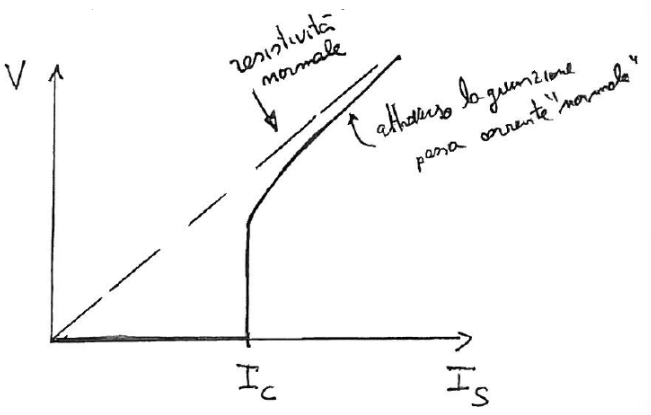
\includegraphics[width=0.35\linewidth]{Immagini - Capitolo 2/effetto Josephson DC.png}
    \caption{andamento di $\Delta V$ alla giunzione in funzione di $I_S$.}
    \label{fig: effetto Josephson DC}
\end{figure}
Fintanto che la corrente è minore del valore critico $I_C$ non si osserva sperimentalmente alcuna differenza di potenziale alla giunzione, tuttavia incrementando l'intensità della corrente oltre $I_C$ la differenza di potenziale balza ad un valore finito, dipendente dalle caratteristiche della giunzione stessa, conseguente in un passaggio di corrente normale. Nel caso in cui $I_S > I_C$ però Josephson scoprì anche una seconda conseguenza dell'effetto tunnel della giunzione: una differenza di potenziale tra i due superconduttori implica che le funzioni d'onda diventano dipendenti dal tempo. Integrando quindi la seconda equazione del sistema \eqref{eq: equazioni effetto Josephson} si ha 
\begin{equation}
    \theta_2 - \theta_1 = \frac{2e\Delta V}{\hbar}t + \theta_0 = \omega_jt + \theta_0.
\end{equation}
Quindi, la differenza di fase cresce linearmente nel tempo e si ha che la corrente è
\begin{equation}
    I_N = I_C\sin{(\omega_jt + \theta_0)}.
\end{equation}
Questo fenomeno invece prende il nome di ``effetto Josephson in AC''. La frequenza $\nu_j \equiv \omega_j/2\pi$ è molto elevata $\nu_j \simeq \SI{48}{\giga\hertz}$ per $\Delta V = \SI{100}{\micro\volt}$. 
\begin{figure}[h]
    \centering
    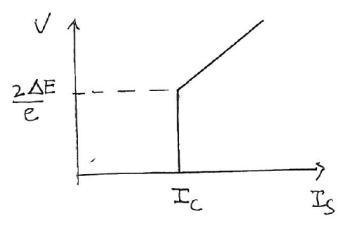
\includegraphics[width=0.35\linewidth]{Immagini - Capitolo 2/effetto Josephson giunzione ideale.png}
    \caption{andamento di $\Delta V$ in funzione di $I_S$ per una giunzione ideale.}
    \label{fig: effetto Josephson giunzione ideale}
\end{figure}

A temperatura $T = \SI{0}{\kelvin}$, in una giunzione ideale, ci si aspetta un comportamento del tipo mostrato in figura \ref{fig: effetto Josephson giunzione ideale}, dove $\Delta E$ è l'energia necessaria per rompere una coppia di Cooper e dove:
\begin{enumerate}
    \item per $I_S < I_C$ la corrente attraverso la giunzione è una supercorrente che non genera una differenza di potenziale;
    \item per $I_S > I_C$ la corrente attraverso la giunzione è una corrente normale, per cui le coppie di Cooper si spezzano.
\end{enumerate}

\subsection{Interferenza quantistica}
L'effetto Josephson è un elemento chiave in molte applicazioni riguardanti l'informatica quantistica. Uno tra i dispositivi più semplici da realizzare è l'anello SQUID (Supeconducting QUantum Interference Device), che consiste in un anello superconduttivo su cui vengono applicate due giunzioni di Josephson, con ognuna delle metà è connessa da un cavo esterno, come mostrato in figura \ref{fig: SQUID}. Le correnti attraverso le giunzioni sono
\begin{equation}
    \begin{cases}
        I_1 = I_{C_1}\sin{\Delta\theta_1} \\
        I_2 = I_{C_2}\sin{\Delta\theta_2} 
    \end{cases},\quad \Delta\theta_i = \theta_{i,R} - \theta_{i,L},\, i = \{1,2\}.
\end{equation}
\begin{figure}[h]
    \centering
    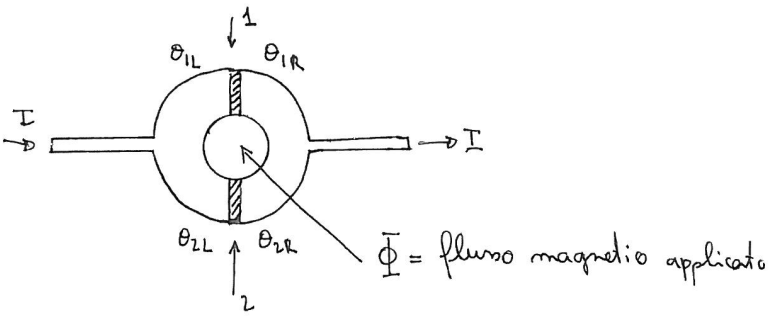
\includegraphics[width=0.6\linewidth]{Immagini - Capitolo 2/SQUID.png}
    \caption{diagramma circuitale dello SQUID.}
    \label{fig: SQUID}
\end{figure}

Supponendo che le giunzioni siano perfettamente identiche, cioè che $I_{C_1} = I_{C_2}$, si ha
\begin{equation}
\label{eq: corrente dello SQUID per giunzioni identiche}
    I = I_C[\sin{(\Delta\theta_1)} + \sin{(\Delta\theta_2)}] = 2I_C\cos{\bigg(\frac{\Delta\theta_1 - \Delta\theta_2}{2}\bigg)}\sin{\bigg(\frac{\Delta\theta_1 + \Delta\theta_2}{2}\bigg)}.
\end{equation}
Se le due giunzioni sono perfettamente bilanciate, applicando una corrente $I < I_C$ ci si aspetta una differenza di fase identica, ossia $\Delta\theta_1 = \Delta\theta_2$, con 
\begin{equation}
    \Delta\theta = \sin^{-1}{\bigg(\frac{I}{2I_C}\bigg)} \neq 0.
\end{equation}
Tuttavia, questo è vero solo se non è presente un campo magnetico all'interno dell'anello. In questo caso la differenza $\Delta\theta_1 - \Delta\theta_2$ dipende dal flusso magnetico $\Phi$ attraverso il dispositivo. Per determinare questa quantità si procede in modo analogo a quanto fatto per la quantizzazione del flusso di campo magnetico per un superconduttore toroidale. Si considerano quindi due cammini $L_1$ ed $L_2$ all'interno del superconduttore dove $\vB = \vo$ e $\vJ_S = \vo$, come mostrato in figura \ref{fig: SQUID calcolo}. 
\begin{equation}
    \begin{cases}
        \theta_{1,R} - \theta_{2,R} = \dfrac{2e}{\hbar}\displaystyle\int_{L_1}\vA \cdot d\vl \\
        \theta_{2,L} - \theta_{1,L} = \dfrac{2e}{\hbar}\displaystyle\int_{L_2}\vA \cdot d\vl
    \end{cases},
\end{equation}
la cui somma risulta in
\begin{equation}
\label{eq: differenza di fase dello SQUID}
    \begin{split}
        \theta_{1,R} - \theta_{2,R} + \theta_{1,L} - \theta_{2,L} &= \frac{2e}{\hbar}\oint\vA \cdot d\vl \\
        \Delta\theta_1 - \Delta\theta_2 &= \frac{2e}{\hbar}\Phi \\
        &= \frac{2\pi\Phi}{\Phi_0}.
    \end{split}
\end{equation}
\begin{figure}[h]
    \centering
    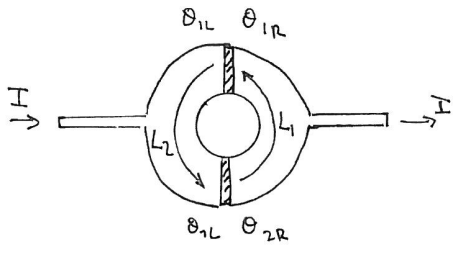
\includegraphics[width=0.5\linewidth]{Immagini - Capitolo 2/SQUID calcolo.png}
    \caption{scelta dei due percorsi per il calcolo della corrente nello SQUID.}
    \label{fig: SQUID calcolo}
\end{figure}

Sostituendo quanto trovato in \eqref{eq: differenza di fase dello SQUID} nell'equazione della corrente \eqref{eq: corrente dello SQUID per giunzioni identiche} si ha
\begin{equation}
    I = 2I_C\sin{\bigg(\frac{\Delta\theta_1 + \Delta\theta_2}{2}\bigg)}\cos{\bigg(\frac{\pi\Phi}{\Phi_0}\bigg)},
\end{equation}
per cui la corrente critica è
\begin{equation}
    I_C(\Phi) = 2I_C\bigg|\cos{\bigg(\frac{\pi\Phi}{\Phi_0}\bigg)}\bigg|.
\end{equation}
L'andamento della corrente critica $I_C(\Phi)$ è mostrato in figura \ref{fig: IC SQUID.png}. Si noti che per $I_C = 0$, una piccolissima corrente $I$ genera una differenza di potenziale ai capi della giunzione. Questo dispositivo permette di misurare piccolissime variazioni di flusso del campo magnetico, con precisione fino a variazioni del campo magnetico nell'ordine di $\SI{e-10}{\tesla}$ attraverso la misura di differenza di potenziale ai capi delle giunzioni quando $I_C \simeq 0$ e $I_C \neq 0$.
\begin{figure}[h]
    \centering
    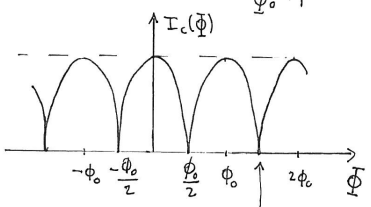
\includegraphics[width=0.5\linewidth]{Immagini - Capitolo 2/IC SQUID.png}
    \caption{andamento della corrente critica $I_C(\Phi)$ dello SQUID.}
    \label{fig: IC SQUID.png}
\end{figure}

\section{Modello di Cooper}
Nonostante il modello di Landau e Ginzburg nonostante sia una teoria fenomenologica che descrive con grande successo molti aspetti e proprietà dei superconduttori, il grande limite di questa teoria tuttavia è la mancata spiegazione dell'origine microscopica del fenomeno di superconduttività. A completare e generalizzare la teoria di Landau e Ginzburg furono Bardeen, Cooper e Schiffer con la loro teoria BCS che provvedeva una spiegazione della superconduttività a livello microscopico prevedendo quantitativamente molte delle proprietà dei superconduttori ``classici''.

Un anno prima della pubblicazione della teoria BCS, Cooper dimostrò che lo stato fondamentale normale di un gas di elettroni è instabile rispetto alla formazione di ``stati legati'' di coppie di elettroni, dove la coppia non è legata nel modo usuale ma lo è a causa delle presenza di un ``mare'' di Fermi, l'elemento chiave per l'esistenza di questo stato; inoltre, in realtà tale stato è a molti elettroni. Alla temperatura $T = \SI{0}{\kelvin}$, nello stato fondamentale normale, tutti gli orbitali macroscopici degli elettroni in un metallo sono occupati fino a $E < \epsilon_F$, mentre i restanti sono vuoti. L'idea di Cooper è di considerare un mare di Fermi ``congelato'' più una coppia di elettroni con energia $E > \epsilon_F$ e con un potenziale efficace a due corpi attrattivo $U(\vr_1,\vr_2) < 0$. Cooper immaginava quindi un'interazione molto debole tra gli elettroni con $U(\vr_1,\vr_2) \simeq 0$; in queste condizioni ci si aspetterebbe che l'eccesso di energia cinetica $\Delta E_K = (E_{K_1} + E_{K_2} -2\epsilon_F) > 0$ non possa essere compensato dalla diminuzione di energia potenziale $\Delta U = 0$. 

Per capire se questo è il caso, si parte dall'equazione di Schr\"odinger corrispondente
\begin{equation}
\label{eq: equazione di Schrodinger BCS completa}
    \bigg[-\frac{\hbar^2}{2m}(\nabla^2_1 + \nabla_2^2) + U(\vr_1,\vr_2)\bigg]\psi(\vr_1,\vr_2) = (\Delta E + 2\epsilon_F)\psi(\vr_1,\vr_2).
\end{equation}
La parte della funzione d'onda $\psi(\vr_1,\vr_2)$ legata allo spin può essere o nello stato di singoletto o in quello di tripletto; tuttavia, maggior parte dei superconduttori le coppie di Cooper corrispondono a stati di singoletto
\begin{equation}
    \chi_{\sigma_1,\sigma_2} = \frac{1}{\sqrt{2}}(\ket{\upa\doa} - \ket{\doa\upa}),
\end{equation}
la quale è antisimmetrica per lo scambio degli elettroni, ossia degli indici $1 \leftrightarrow 2$, mentre $\psi(\vr_1,\vr_2)$ è simmetrica dato che le particelle in questione sono appunto identiche. L'autovalore $\Delta E$ è definito relativamente al livello di Fermi $2\epsilon_F$. Si consideri il sistema di coordinate del centro di massa
\begin{equation}
    \begin{cases}
        \vR = \dfrac{1}{2}(\vr_1 + \vr_2) \\
        \vr = \vr_1 - \vr_2
    \end{cases},
\end{equation}
così da riscrivere l'equazione di Schr\"odinger come
\begin{equation}
   \bigg[-\frac{\hbar^2}{4m}\nabla^2_R - \frac{2\hbar^2}{2m}\nabla^2_r\bigg]\psi(\vR,\vr) + U(\vr)\psi(\vR,\vr) = (\Delta E + 2\epsilon_F)\psi(\vR,\vr).
\end{equation}
Separando adesso la funzione d'onda nelle sue variabili ponendo
\begin{equation}
    \psi(\vR,\vr) = \Phi(\vR)\psi(\vr),\quad \Phi(\vR) = e^{i(\vQ\cdot \vR)}
\end{equation}
e considerando al momento solo lo stato con $\vQ = \vo$, si rimane con
\begin{equation}
\label{eq: equazione di Schrodinger BCS psi(r)}
   \bigg[- \frac{2\hbar^2}{2m}\nabla^2_r + U(\vr)\bigg]\psi(\vr) = (\Delta E + 2\epsilon_F)\psi(\vr),
\end{equation}
gli stati con $\vQ \neq \vo$ sono invece necessari per descrivere un flusso di corrente stazionario. Si supponga adesso che la funzione d'onda $\psi(\vr)$ sia una certa sovrapposizione su tutti gli stati
\begin{equation}
    \psi(\vr) = \frac{1}{\sqrt{V}}\sum_{k  > k_F}a_ke^{i(\vk \cdot \vr)},
\end{equation}
dove la somma è fatta su tutti i numeri d'onda $k \equiv |\vk| > k_F$. Sostituendo quest'ultima relazione nell'equazione \eqref{eq: equazione di Schrodinger BCS psi(r)} si ha
\begin{equation}
    \sum_{k > k_F}[2(\epsilon_k - \epsilon_F) - \Delta E]a_ke^{i(\vk \cdot \vr)} + \sum_{k > k_F}U(\vr)a_ke^{i(\vk \cdot \vr)} = 0,\quad \epsilon_k \equiv \frac{\hbar^2k^2}{2m}
\end{equation}
che se moltiplicata per $e^{-i(\vk' \cdot \vr)}/V$ ed integrata su $\vr$ porta a
\begin{equation}
    \begin{split}
        0 &= [2(\epsilon_{k'} - \epsilon_F) - \Delta E]a_{k'} + \sum_{k > k_F}a_k\int\frac{d^3r}{V}U(\vr)e^{i(\vk - \vk')\cdot \vr} \\
        &= [2(\epsilon_{k'} - \epsilon_F) - \Delta E]a_{k'} + \sum_{k > k_F}a_kU(\vk,\vk'),
    \end{split}
\end{equation}
dove $U(\vk,\vk')$ è la trasformata di Fourier di $U(\vr)$, ossia
\begin{equation}
    U(\vk,\vk') = \frac{1}{V}\int d^3r\,e^{i(\vk - \vk')\cdot \vr}U(\vr).
\end{equation}
Per procedere si deve necessariamente supporre la forma del potenziale di interazione, in questo caso
\begin{equation}
    U(\vk,\vk') =
    \begin{cases}
        -V_0,\quad 0 \le \epsilon_{k,k'} - \epsilon_F \le \hbar\omega_D\\
        0,\quad \mathrm{altrimenti}
    \end{cases},
\end{equation}
dove $\hbar\omega_D$ è un valore di soglia che formalizza l'assunzione che solo gli elettroni in una banda attorno al livello di Fermi contribuiscono al processo di scattering $(\vk_i,\vk'_i) \to (\vk_f,\vk'_f)$, il quale è possibile solo se $|\vk_i|$, $|\vk_i'|$, $|\vk_f|$ e $|\vk_f'|$ sono maggiori di $k_F$. In particolare, $\hbar\omega_D$ è l'energia di Debye, ossia la massima energia che può acquisire un fonone in un reticolo. Questo riflette l'idea che l'interazione tra elettroni avvenga attraverso lo scambio di fononi reticolari. Si trova allora
\begin{equation}
    \sum_{k > k_F}a_kU(\vk,\vk') = 
    \begin{cases}
        -V_0\nsump{k > k_F}a_k,\quad 0 \le \epsilon_{k'} - \epsilon_F \le \hbar\omega \\
        0,\quad \mathrm{altrimenti}
    \end{cases},
\end{equation}
quindi si ha
\begin{align}
    [2(\epsilon_{k'} - \epsilon_F) - \Delta E]a_{k'} - V_0\sump_{k > k_F}a_k &= 0 \\
    a_{k'} &= \frac{V_0\nsump{k > k_F}a_k}{2(\epsilon_{k'} - \epsilon_F) - \Delta E},
\end{align}
da cui, sommando su $k'$, si trova
\begin{equation}
    \frac{1}{V_0} = \sump_{k > k_F}\frac{1}{2(\epsilon_k - \epsilon_F) - \Delta E}.
\end{equation}
La somma può essere trasformata in un integrale se si introduce la densità degli stati $D(\epsilon_k)$, così da avere
\begin{equation}
    \int_{\epsilon_F}^{\epsilon_F + \hbar\omega_D}d\epsilon\,\frac{V_0D(\epsilon)}{2(\epsilon - \epsilon_F) - \Delta E} = 1.
\end{equation}
Considerando adesso il limite in cui $\hbar\omega_D \ll 1$, allora $D(\epsilon) \simeq D(\epsilon_F)$ e l'integrale si riduce all'equazione
\begin{equation}
    \begin{split}
        \frac{V_0}{2}D(\epsilon_F)\log{[2(\epsilon - \epsilon   _F) - \Delta E]}|_{\epsilon_F}^{\epsilon_F + \hbar\omega_D} &= \frac{V_0}{2}D(\epsilon_F)\log{\bigg(\frac{\Delta E - 2\hbar\omega_D}{\Delta E}\bigg)} \\
        &\simeq 1,
    \end{split}
\end{equation}
che risolvendo per $\Delta E$ restituisce
\begin{equation}
\label{eq: differenza di energia stati BCS}
    \Delta E = -\frac{2\hbar\omega_D}{e^{2/V_0D(\epsilon_F)} - 1}.
\end{equation}
In particolare, nel limite di interazione debole $V_0D(\epsilon_F) \ll 1$, l'esponenziale domina a denominatore risultando in 
\begin{equation}
\label{eq: differenza di energia stati BCS limite interazione debole}
    \Delta E \simeq -2\hbar\omega_De^{-2/V_0D(\epsilon_F)},
\end{equation}
che se sostituito in $\Delta E + 2\epsilon_F$ porta al risultato ottenuto da Cooper
\begin{equation}
    \Delta E + 2\epsilon_F \simeq 2\epsilon_F - 2\hbar\omega_De^{-2/V_0D(\epsilon_F)} < 2\epsilon_F.
\end{equation}
Esiste quindi uno stato ``legato'' con energia negativa, rispetto alla superficie di Fermi costituito da elettroni con $|\vk| > k_F$, cioè con energia cinetica superiore a $\epsilon_F$. Lo stato composto da elettroni accoppiati in questo modo avrà sempre un'energia minore di quella dello stato fondamentale, anche per valori di $V_0$ arbitrariamente piccoli. Questo è il motivo per cui si considera lo stato fondamentale normale instabile rispetto alla formazione di coppie di Cooper. Inoltre, questo risultato non può essere ottenuto con metodi perturbativi sviluppando in potenze di $V_0$. L'espressione ottenuta per $\Delta E$ nell'equazione \eqref{eq: differenza di energia stati BCS limite interazione debole} mette in evidenza una gerarchia di energia $\epsilon_F \gg \hbar\omega_D \gg |\Delta E|$, assumendo poi che $|\Delta E| \simeq kT_c$, allora tale gerarchia spiega come mai la transizione a superconduttore avviene a temperature molto basse rispetto alla temperatura di Debye $T_D = \hbar\omega_D/k$. 

\paragraph{Effetto isotropico.} L'idea che 
l'attrazione tra elettroni sia conseguenza dell'interazione elettrone-fonone è confermata dall'effetto isotropico, che consiste nella relazione $T_c \propto m^{-\alpha}$, dove $m$ è la massa dello ione che costituisce, il reticolo cristallino. La teoria delle vibrazioni nei cristalli prevede che la frequenza di vibrazione $\omega(q)$ siano tutte proporzionali a $\sqrt{K/m}$, dove $K$ è la costante elastica del potenziale classico di interazione elastica fra tutti i primi vicini del reticolo. Quindi, poiché
\begin{equation}
    kT_c \simeq \Delta E \propto \hbar\omega_D \propto \sqrt{\frac{K}{m}},
\end{equation}
si trova immediatamente che $T_c \propto m^{-1/2}$, che corrisponde al valore osservato dell'esponente critico per i metalli puri. L'ipotesi che le interazioni elettrone-nucleo fossero importanti è dovuta a Fr\"olich: al passaggio di un elettrone. il reticolo tende a deformarsi creando un eccesso di carica totale che può attrarre un secondo elettrone, come mostrato in figura \ref{fig: carica di un reticolo}. In particolare, gli elettroni interagiscono a distanza attraverso il reticolo e tale interazione è attrattiva e mediata dallo scambio di fononi. Nei superconduttori ad alta temperatura l'effetto isotropico non si verifica, ciò potrebbe indicare che non sono i fononi i responsabili del gap di energia.
\begin{figure}[h]
    \centering
    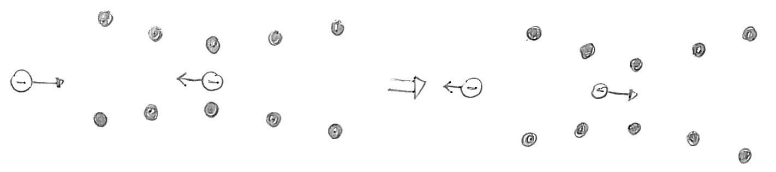
\includegraphics[width=0.6\linewidth]{Immagini - Capitolo 2/carica di un reticolo.png}
    \caption{deformazione della distribuzione di carica di un reticolo cristallino al passaggio di un elettrone.}
    \label{fig: carica di un reticolo}
\end{figure}

\subsection{Stato fondamentale}
Più sopra si è dimostrato che il mare di Fermi è instabile per la creazione di coppie di Cooper quando l'interazione effettiva tra due elettroni è attrattiva. Ci si aspetta di conseguenza una condensazione di coppie di Cooper fino a quando non si raggiunge uno stato di equilibrio. Questo avviene dopo che lo stato di Fermi è cambiato così tanto che l'aggiunta di un'altra coppia di Cooper non è più associata ad una diminuzione dell'energia. Per studiare uno stato interagente di questo tipo si deve introdurre il formalismo della seconda quantizzazione per i fermioni seguendo un procedimento del tutto simile al caso bosonico, con la differenza che questa volta si introduce una relazione di anti-commutazione
\begin{equation}
    \acomm{\hata}{\hatb} = \hata\hatb + \hatb\hata,
\end{equation}
passando così dalla statistica di Bose-Einstein a quella di Fermi-Dirac. Fin dal principio è conveniente lavorare nello spazio degli impulsi introducendo gli operatori di creazione $\hatC^\dg_{k\sigma}$ e di distruzione $\hatC_{k\sigma}$ che, rispettivamente, creano e distruggono un fermione con momento $\vk$ e terza componente di spin $\sigma = \{\upa,\doa\}$. Indicando con $\kO$ lo stato di vuoto corrispondente alla totale assenza di fermioni in modo tale che $\hatC_{k\sigma}\kO = 0$, gli operatori $\hatC$ e $\hatC^\dg$ soddisfano le seguenti regole di anticommutazione
\begin{equation}
    \begin{cases}
        \acomm{\hatC_{k\sigma}^\dg}{\hatC_{k'\sigma'}} = \delta_{k,k'}\delta_{\sigma,\sigma'} \\
        \acomm{\hatC_{k\sigma}^\dg}{\hatC^\dg_{k'\sigma'}} = 0 \\
        \acomm{\hatC_{k\sigma}}{\hatC_{k'\sigma'}} = 0
    \end{cases}.
\end{equation}
Applicando l'operatore di creazione $\hatC^\dg$ sullo stato fondamentale $\kO$ si ottiene uno stato 
\begin{equation}
    \hatC^\dg_{k\sigma}\kO = \ket{k\sigma} \equiv \ket{1_{k\sigma}},
\end{equation}
inoltre gli stati a molti elettroni sono automaticamente antisimmetrici per lo scambio delle particelle. Se poi $(k,\sigma) = (k',\sigma')$, allora $\ket{2_{k\sigma}} = -\ket{2_{k\sigma}}$, per cui $\ket{2_{k\sigma}} = 0$, o analogamente
\begin{equation}
    (\hatC^\dg_{k\sigma})^2 = (\hatC_{k\sigma})^2 = 0,
\end{equation}
che corrisponde al principio di esclusione di Pauli in Meccanica quantistica. L'operatore $\hatN_{k\sigma} = \hatC^\dg_{k\sigma}\hatC_{k\sigma}$ è l'operatore ``numero di elettroni'' con impulso $\vk$ e terza componente di spin $\sigma$, il quale soddisfa le seguenti regole di commutazione
\begin{equation}
    \begin{cases}
        \comm{\hatN_{k\sigma}}{\hatC^\dg_{k\sigma}} = \hatC^\dg_{k\sigma}(\hatN_{k\sigma} + 1) \\
        \comm{\hatN_{k\sigma}}{\hatC_{k\sigma}} = \hatC_{k\sigma}(\hatN_{k\sigma} - 1)
    \end{cases}
\end{equation}
e che agisce su uno stato generico $\ket{S}$ come
\begin{equation}
    \hatN_{k\sigma}\ket{S} = 
    \begin{cases}
        0,\quad \ket{S} = \ket{\dots,0_{k\sigma},\dots} \\
        1,\quad \ket{S} = \ket{\dots,1_{k\sigma},\dots}
    \end{cases},
\end{equation}
da cui si deduce anche che $(\hatN_{k\sigma})^2 = \hatN_{k\sigma}$. L'operatore ``numero totale'' di elettroni è dato da
\begin{equation}
    \hatN = \nsum_{k\sigma}\hatN_{k\sigma}.
\end{equation}
\begin{obs}
    In Meccanica quantistica non-relativistica per fermioni, il formalismo della seconda quantizzazione permette di evitare l'introduzione degli ingombranti determinanti di Slater. A fissato numero di particelle i approcci sono perfettamente equivalenti.
\end{obs}
Si introduce adesso la funzione d'onda per la coppia di Cooper come
\begin{equation}
    \psi_{CP} \equiv \psi_\sigma\psi_r = \frac{1}{\sqrt{2}}(\ket{\upa\doa} - \ket{\doa\upa})\psi(\vr_1,\vr_2),
\end{equation}
dove
\begin{equation}
    \psi(\vr_1,\vr_2) = N\sum_{k > k_F}a_ke^{i\vk\cdot(\vr_1 - \vr_2)}.
\end{equation}
Nello spazio degli impulsi con il formalismo della seconda quantizzazione si può scrivere
\begin{equation}
    N\sum_{k > k_F}a_k\ket{1_{k\upa},1_{-k\doa}}_F = N\sum_{k > k_F}a_k\hatC^\dg_{k\upa}\hatC_{-k\doa}\ket{F}.
\end{equation}
Pertanto, conviene introdurre l'operatore di creazione di coppie di Cooper come
\begin{equation}
    \hatP^\dg_k = \hatC^\dg_{k\upa}\hatC^\dg_{-k\doa},\quad \hatP_k = \hatC_{-k\doa}\hatC_{k\upa}.
\end{equation}
Sebbene siano operatori composti da due operatori di tipo fermionico non sono totalmente equivalenti
ad operatori bosonici; valgono infatti le seguenti proprietà di commutazione:
\begin{enumerate}
    \item $\comm{\hatP_k^\dg}{\hatP^\dg_{k'}} = \comm{\hatP_k}{\hatP_{k'}} = 0$;
    \item $(\hatP_k^\dg)^2 = 0$;
    \item usando le espressioni degli operatori di creazione e distruzione fermionici $\hatC_{k\upa}\hatC^\dg_{k\upa} = 1 - \hatC_{k\upa}^\dg\hatC_{k\upa}$ e $\hatC^\dg_{-k\doa}\hatC_{-k\doa} = 1 - \hatC_{-k\doa}\hatC^\dg_{-k\doa}$ si ha
    \begin{equation}
        \begin{split}
            \comm{\hatP_k}{\hatP^\dg_k} &= \hatP_k\hatPT_k - \hatPT_k\hatP_k \\
            &= \hatCT_{-k\doa}\hatC_{k\upa}\hatCT_{k\upa}\hatCT_{-k\doa} - \hatCT_{k\upa}\hatCT_{-k\doa}\hatC_{-k\doa}\hatC_{k\upa} \\ 
            &= (1 - \hatN_{-k\doa} - \hatN_{k\upa}).
        \end{split}
    \end{equation}
\end{enumerate}
Pertanto, gli operatori $\hatP_k$ e $\hatP_k^\dg$ non sono operatori canonicamente commutanti, dato che il loro commutatore è diverso da 1.

Si costruisce adesso lo stato fondamentale $\ket{\psi_{BCS}}$ che descrive il superconduttore a $T = \SI{0}{\kelvin}$ in presenza di un condensato di coppie di Cooper. In analogia con i condensati di Bose-Einstein, Schreiffer propose come stato fondamentale lo stato ``coerente'' definito da
\begin{equation}
    \ket{\psi_{BCS}} = \bar{N}\nprod_k e^{\alpha_k\hatP_k^\dg}\kO,\quad \bar{N},\alpha_k \in \C,
\end{equation}
dove $\alpha_k = \alpha_{-k}$ per ogni $k$ e dove $\bar{N}$ è una costante di normalizzazione. Per il principio di esclusione di Pauli, corrispondente a $(\hatPT_k)^2 = 0$, lo stato coerente appena definito si può espandere come
\begin{equation}
    \ket{\psi_{BCS}} = \bar{N}\nprod_k(1 + \alpha_k\hatP_k^\dg)\kO,
\end{equation}
con i parametri $\{\alpha_k\}$ da fissare per minimizzare l'energia dell'hamiltoniana del modello BCS. Per determinare la costante di normalizzazione $\bar{N}$, sapendo che $\mybraket{\Omega}{\Omega} = 1$, si impone la condizione di normalizzazione $\mybraket{\psi_{BCS}}{\psi_{BCS}} = 1$ che porta a
\begin{equation}
    \begin{split}
        1 &= |\bar{N}|^2\prod_{k,k'}\mybrakett{\Omega}{(1 + \alpha_k^*\hatP_k)(1 + \alpha_{k'}\hatP_{k'}^\dg)}{\Omega} \\
        &= |\bar{N}|^2\prod_{k,k'}(\mybraket{\Omega}{\Omega} + \mybrakett{\Omega}{\alpha_k^*\alpha_{k'}\hatP_k\hatP_{k'}^\dg}{\Omega}) \\
        &= |\bar{N}|^2\prod_{k,k'}(1 + \alpha_k^*\alpha_{k'}\mybrakett{\Omega}{\hatP_k\hatP_{k'}^\dg}{\Omega}) \\
        &= |\bar{N}|^2\nprod_{k}\mybrakett{\Omega}{(1 + \alpha_k^*\hatP_k)(1 + \alpha_k\hatP_k^\dg)}{\Omega} \\
        &= |\bar{N}|^2\nprod_{k}\mybrakett{\Omega}{(1 + |\alpha_k|^2(1 - \hatN_{-k\doa} - \hatN_{k\upa} + \hatP_k^\dg\hatP_k)}{\Omega} \\
        &= |\bar{N}|^2\nprod_{k}(1 + |\alpha_k|^2),
    \end{split}
\end{equation}
da cui si ricava
\begin{equation}
    \bar{N} = \nprod_k\frac{1}{\sqrt{1 + |\alpha_k|^2}},
\end{equation}
dove si sono usate le proprietà degli operatori di creazione e distruzione di coppie di Cooper $\mybrakett{\Omega}{\hatP_{k}\hatP_{k'}^\dg}{\Omega} = \delta_{k,k'}$ e $\mybrakett{\Omega}{\hatP_k}{\Omega} = \mybrakett{\Omega}{\hatP_k^\dg}{\Omega} = 0$. Dunque, lo stato fondamentale è
\begin{equation}
    \ket{\psi_{BCS}} = \nprod_k\bigg(\frac{e^{i\theta_k}}{\sqrt{1 + |\alpha_k|^2}} + \frac{\alpha_ke^{i\theta_k}}{\sqrt{1 + |\alpha_k|^2}}\hatP_k^\dg\bigg)\kO \equiv \nprod_k(u_k^* + v_k^*\hatP_k^\dg)\kO,
\end{equation}
dove si ha una possibile fase globale data da $|u_k|^2 + |v_k|^2 = 1$ con $|u_k|^2 = |u_{-k}|^2$ e $|v_k|^2 = |v_{-k}|^2$. Usando poi il fatto che $\hatP_k\hatP_k^\dg\kO = \kO$, si può riscrivere lo stato fondamentale in termini del livello di Fermi come
\begin{equation}
    \begin{split}
        \ket{\psi_{BCS}} &= \nprod_k(u_k^* + v_k^*\hatP_k^\dg)\prod_{k < k_F}\hatP_k\hatP_k^\dg\kO \\
        &= \nprod_k(u_k^* + v_k^*\hatP_k^\dg)\prod_{k < k_F}\hatP_k\ket{F} \\
        &= \prod_{k > k_F}(u_k^* + v_k^*\hatP_k^\dg)\prod_{k < k_F}[(u_k^* + v_k^*\hatP_k^\dg)\hatP_k]\ket{F} \\
        &= \prod_{k > k_F}(u_k^* + v_k^*\hatP_k^\dg)\prod_{k < k_F}(u_k^*\hatP_k + v_k^*)\ket{F},
    \end{split}
\end{equation}
dove il primo termine restituisce il numero di coppie di Cooper, mentre il secondo il numero di lacune di Cooper. L'andamento del numero di fermioni con momento $\vk$ e terza componente di spin $\sigma$ è mostrato in figura \ref{fig: numero fermioni BCS}.
\begin{figure}[h]
    \centering
    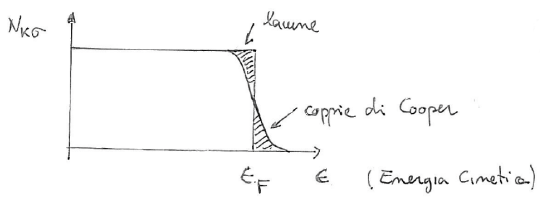
\includegraphics[width=0.6\linewidth]{Immagini - Capitolo 2/numero fermioni BCS.png}
    \caption{andamento del numero di fermioni nel superconduttore in funzione dell'energia cinetica $\epsilon$.}
    \label{fig: numero fermioni BCS}
\end{figure}

Il prossimo passo è quello di introdurre l'hamiltoniana del modello BCS. L'hamiltoniana di partenza ha la stessa forma di quella di Gross-Pitaevskii con potenziale di interazione a delta di Dirac per descrivere i gas diluiti a bassa temperatura, con la differenza che ora si devono considerare gli operatori fermionici, per cui 
\begin{equation}
    \hatH_{BCS} = \sump_{k,\sigma}\epsilon_k\hatC^\dg_{k\sigma}\hatC_{k\sigma} - |g|\sump_{\substack{k_1,k_2 \\ \sigma_1,\sigma_2 \\
    q}}\hatC^\dg_{k_1 + q,\sigma_1}\hatC^\dg_{k_2 - q,\sigma_2}\hatC_{k_1\sigma_1}\hatC_{k_2\sigma_2},
\end{equation}
dove l'indice della somma $\Sigma'$ è ristretto a $\epsilon_F - \hbar\omega_D \le \epsilon_k \le \epsilon_F + \hbar\omega_D$. Se ora si assume che l'interazione rilevante per la superconduttività coinvolga solo le coppie di Cooper, l'hamiltoniana diventa
\begin{equation}
    \hatH_{BCS} = \sump_{k,\sigma}\epsilon_k\hatN_{k\sigma} - |g|\sump_{k,k'}\hatP^\dg_k\hatP_{k'},\quad \epsilon_k = \frac{\hbar^2k^2}{2m}.
\end{equation}
Tuttavia, questa hamiltoniana non può essere diagonalizzata in modo esatto. Pertanto, si deve usare il fatto che la funzione d'onda $\ket{\psi_{BCS}}$ contiene i parametri $u_k^*$ e $v_k^*$ che possono essere trattati con il metodo variazionale, i quali vengono fissati richiedendo che $E = \mybrakett{\psi_{BCS}}{\hatH}{\psi_{BCS}}$ sia minima con il vincolo che $N \equiv \mybrakett{\psi_{BCS}}{\hatN}{\psi_{BCS}}$ sia fissato e valga la condizione $|u_k|^2 + |v_k|^2 = 1$. Si considera in primis il termine cinetico
\begin{equation}
    \hatT \equiv \sump_{k,\sigma}\epsilon_k\hatN_{k\sigma} = \sump_{k,\sigma}\epsilon_k(\hatN_{k\upa} + \hatN_{-k\doa}).
\end{equation}
Sapendo che $\hatN^\dg_{k\upa} = \hatN_{k\upa}$, si calcola
\begin{equation}
    \begin{split}
        \vmedio{\hatN_{k\upa}}_{BCS} = \vmedio{\hatC^\dg_{k\upa}\hatC_{k\upa}}_{BCS} &= \mybrakett{\Omega}{(u_k + v_k\hatP_k)\hatN_{k\upa}(u_k^* + v_k^*\hatP_k^\dg)}{\Omega} \\
        &= |u_k|^2\cancelto{0}{\mybrakett{\Omega}{\hatN_{k\upa}}{\Omega}} + |v_k|^2\mybrakett{\Omega}{\hatP_k\hatN_{k\upa}\hatPT_k}{\Omega} \\
        &= |v_k|^2\mybrakett{\Omega}{\hatP_k\hatN_{k\upa}\hatP_k^\dg}{\Omega} \\
        &= |v_k|^2,
    \end{split}
\end{equation}
dove si è usata la proprietà $\comm{\hatN_{k\upa}}{\hatP_k^\dg} = \hatP_k^\dg$. In modo simile, si può ricavare $\vmedio{\hatN_{-k\doa}}_{BCS} = |v_k|^2$. Dunque, il valor medio $N$ è dato da
\begin{equation}
    N \equiv \mybrakett{\psi_{BCS}}{\hatN_{k\sigma}}{\psi_{BCS}} = 2\nsump{k}|v_k|^2 = \nsump{k}(|v_k|^2 - |u_k^2| + 1),
\end{equation}
per cui 
\begin{equation}
    \bigvmedio{\sump_{k,\sigma}\epsilon_k\hatC^\dg_{k\sigma}\hatC_{k\sigma}}_{BCS} = 2\nsump{k}\epsilon_k|v_k|^2 = \nsump{k}\epsilon_k(|v_k|^2 - |u_k^2| + 1).
\end{equation}
Per quanto riguarda la parte di interazione 
\begin{equation}
    \begin{split}
        \vmedio{\hatPT_k\hatP_{k'}}_{BCS} &= \mybrakett{\Omega}{(u_{k'} + v_{k'}\hatP_{k'})(u_k + v_k\hatP_k)(\hatPT_k\hatP_{k'}) \\ 
        &\times (u^*_{k'} + v^*_{k'}\hatPT_{k'})(u^*_k + v_k^*\hatPT_k)}{\Omega} \\
        &= \mybrakett{\Omega}{\hatP_k\hatPT_k\hatP_{k'}\hatPT_{k'}}{\Omega}v_kv_{k'}^*u_{k'}u_k^* \\
        &= v_kv_{k'}^*u_{k'}u_k^*.
    \end{split}
\end{equation}
Quindi, il valore medio dell'hamiltoniana espresso in funzione dei parametri $v_k$ e $u_k$ è
\begin{equation}
    \begin{split}
        \vmedio{\hatH}_{BCS} \equiv E &= 2\nsump{k}\epsilon_k|v_k|^2 - |g|\sump_{k,k'}v_kv_{k'}^*u_{k'}u_k^* \\
        &= \nsump{k}\epsilon_k(|v_k|^2 - |u_k|^2 + 1) - |g|\sump_{k,k'}v_kv_{k'}u_{k'}u_k^*.
    \end{split}
\end{equation}
Le condizioni di minimo sono
\begin{equation}
    \begin{cases}
        \dfrac{\p}{\p u_k^*}\bigg[E - \mu N + \nsump{k}E_k(|u_k|^2 + |v_k|^2 - 1)\bigg] = 0 \\[2ex]
        \dfrac{\p}{\p v_k^*}\bigg[E - \mu N + \nsump{k}E_k(|u_k|^2 + |v_k|^2 - 1)\bigg] = 0
    \end{cases},
\end{equation}
dove $\mu$ è il moltiplicatore di Lagrange di $N$, mentre $E_k$ è quello dei vincoli $|u_k|^2 + |v_k|^2 = 1$. Quindi, ponendo $\Sigma \equiv E_k(|u_k|^2 + |v_k|^2 - 1)$, computando i vari termini nella prima equazione del sistema
\begin{equation}
    \mu\frac{\p N}{\p u_k^*} = -\mu u_k, \quad \frac{\p \Sigma}{\p u_k^*} = E_ku_k,\quad \frac{\p E}{\p u_k^*} = -\epsilon_ku_k - |g|v_k\nsump{k'}v_{k'}^*u_{k'}
\end{equation}
e per la seconda equazione del sistema
\begin{equation}
    \mu\frac{\p N}{\p v_k^*} = \mu v_k, \quad \frac{\p \Sigma}{\p v_k^*} = E_kv_k,\quad \frac{\p E}{\p v_k^*} = -\epsilon_kv_k - |g|u_k\nsump{k'}v_{k'}u_{k'}^*,
\end{equation}
si ottiene
\begin{equation}
    \begin{cases}
        (\epsilon_k - \mu)u_k + \Delta v_k = E_ku_k \\
        \Delta^*u_k - (\epsilon_k - \mu)v_k = E_kv_k
    \end{cases},
\end{equation}
dove si sono introdotti i parametri di gap
\begin{equation}
\label{eq: parametri di gap BCS definizione}
    \Delta \equiv |g|\nsump{k}v_k^*u_k,\quad \Delta^* \equiv |g|\nsump{k}v_ku_k^*.
\end{equation}
Nella teoria BCS, il parametro $\Delta$ ha un importante significato fisico; infatti, considerando il valore medio dell'operatore $\hatP_k$ sullo stato fondamentale 
\begin{equation}
    \begin{split}
        \vmedio{\hatP_k}_{BCS} &= \mybrakett{\Omega}{(u_k + v_k\hatP_k)\hatP_k(u_k^* + v_k^*\hatPT_k)}{\Omega} \\
        &= u_kv_k^*\mybrakett{\Omega}{\hatP_k\hatPT_k}{\Omega} \\
        &= u_kv_k^*
    \end{split}
\end{equation}
si trova che 
\begin{equation}
    \Delta = |g|\nsump{k}\vmedio{\hatP_k}_{BCS},
\end{equation}
ossia il parametro $\Delta$ è legato al valore di aspettazione delle coppie di Cooper sullo stato fondamentale $\ket{\psi_{BCS}}$. Per trovare $\Delta$ bisogna risolvere il sistema lineare
\begin{equation}
    \begin{pmatrix}
        \epsilon_k - \mu & \Delta \\
        \Delta^* & -\epsilon_k + \mu
    \end{pmatrix}
    \begin{pmatrix}
        u_k \\
        v_k
    \end{pmatrix} \equiv M(\Delta)
    \begin{pmatrix}
        u_k \\
        v_k
    \end{pmatrix} = E_k
    \begin{pmatrix}
        u_k \\
        v_k
    \end{pmatrix},
\end{equation}
il quale ha soluzione non banale se e solo se 
\begin{equation}
    \det{[M(\Delta) - \MI E_k]} = \det
    \begin{pmatrix}
        \epsilon_k - \mu - E_k & \Delta \\
        \Delta^* & -\epsilon_k + \mu - E_k
    \end{pmatrix} = 0,
\end{equation}
la quale porta all'equazione di secondo grado $E_k^2 - (\epsilon_k - \mu)^2 - |\Delta|^2 = 0$, da cui a sua volta si trovano gli autovalori 
\begin{equation}
    \begin{cases}
        E_k = \sqrt{(\epsilon_k - \mu)^2 + |\Delta|^2} \\
        E_k' = -E_k
    \end{cases}.
\end{equation}
Quindi, si nota che $E_k$ corrisponde all'energia di un quasi-elettrone mentre $E_k'$ corrisponde all'energia di una quasi-lacuna. Per trovare ora un'equazione per $\Delta$ si parte dalle equazioni
\begin{equation}
    \begin{cases}
        v_k^*[(\epsilon_k - \mu)u_k + \Delta v_k] = E_ku_kv_k^* \\
        u_k[\Delta u_k^* - (\epsilon_k - \mu)v_k^*] = E_kv_k^*u_k
    \end{cases}
\end{equation}
la cui somma porta alla relazione
\begin{equation}
\label{eq: relazione parametro di gap BCS}
    u_kv_k^* = \frac{\Delta}{2E_k}
\end{equation}
ed anche alle relazioni
\begin{equation}
    \begin{cases}
        |v_k|^2 = \dfrac{1}{2}\bigg(1 - \dfrac{\epsilon_k - \mu}{E_k}\bigg) \\[2ex]
        |u_k|^2 = \dfrac{1}{2}\bigg(1 + \dfrac{\epsilon_k - \mu}{E_k}\bigg)
    \end{cases}.
\end{equation}
Considerando per prima la relazione \eqref{eq: relazione parametro di gap BCS} e usando la definizione del parametro di gap introdotta in equazione \eqref{eq: parametri di gap BCS definizione} si ottiene
\begin{equation}
    \frac{|g|}{2}\nsump{k}\frac{1}{[(\epsilon_k - \mu)^2 + |\Delta|^2]^{1/2}} = 1.
\end{equation}
Quest'ultima equazione è centrale nella teoria BCS in quanto determina il parametro di gap $|\Delta|$ a $T = \SI{0}{\kelvin}$. Per valutare questa quantità, si può operare la sostituzione
\begin{equation}
    \nsump{k} \to D(\epsilon_F)\int_{-\hbar\omega_D}^{\hbar\omega_D}d\epsilon = 2D(\epsilon_F)\int_0^{\hbar\omega_D}d\epsilon,\quad \epsilon \equiv \epsilon_k - \mu,
\end{equation}
passando così dal discreto ad un intervallo continuo assumendo che i livelli energetici siano molto densi; in questo modo si ottiene
\begin{equation}
    \Lambda\int_0^{\hbar\omega_D}\frac{d\epsilon}{[\epsilon^2 + |\Delta|^2]^{1/2}} = 1,\quad \Lambda \equiv |g|D(\epsilon_F).
\end{equation}
Per risolvere questo integrale si utilizza la formula generale
\begin{equation}
    \int_0^b \frac{dx}{\sqrt{x^2 + a^2}} = -\frac{1}{2}\log{(a^2)} + \log{(b + \sqrt{a^2 + b^2})},
\end{equation}
che in questo caso restituisce
\begin{equation}
    \begin{split}
        1 &= \Lambda\bigg\{-\frac{1}{2}\log|\Delta|^2 + \log{\bigg[\hbar\omega_D + \sqrt{|\Delta|^2 + (\hbar\omega_D)^2}\bigg]}\bigg\} \\
        &\simeq \Lambda\log{\bigg(\frac{2\hbar\omega_D}{|\Delta|}\bigg)},
    \end{split}
\end{equation}
da cui si ricava finalmente la formula per il parametro di gap a temperatura $T = \SI{0}{\kelvin}$ della teoria BCS
\begin{equation}
\label{eq: formula parametro gap a T=0 BCS}
    |\Delta| \simeq 2\hbar\omega_De^{-1/\Lambda}.
\end{equation}
Si possono anche calcolare gli autovettori della matrice $M(\Delta)$ corrispondenti agli autovalori $E_k$ ed $E_k'$ rispettivamente che risultano essere i vettori $\begin{pmatrix} u_k & -v_k\end{pmatrix}^T$ e $\begin{pmatrix} v_k^* & -u_k^*\end{pmatrix}^T$. Inoltre, dalla relazione \eqref{eq: relazione parametro di gap BCS} si può dedurre che gli autovettori della matrice $M(-\Delta)$ sono $\begin{pmatrix} u_k & -v_k\end{pmatrix}^T$ e $\begin{pmatrix} v_k^* & u_k^*\end{pmatrix}^T$.

\subsection{Stati eccitati}
Avendo ottenuto $\ket{\psi_{BCS}}$ tramite metodi variazionali, il passo successivo è quello di fare predizioni sulle proprietà fisiche dei superconduttori. Il metodo utilizzato per trovare gli stati eccitati è simile a quello usato nei superfluidi attraverso la trasformazione di Bogoljubov. L'idea è di considerare $\ket{\psi_{BCS}}$ come stato di riferimento e di considerare eccitazioni a bassa energia relativamente a questo stato. Il metodo è basato sull'approssimazione 
\begin{equation}
    \hatPT_k\hatP_{k'} \simeq \vmedio{\hatPT_k}_{BCS} \hatP_{k'} + \hatPT_k\vmedio{\hatP_{k'}}_{BCS},
\end{equation}
con la quale si ottiene l'hamiltoniana
\begin{equation}
    \hatH  = \sum_{k,\sigma}(\epsilon_k - \mu)\hatCT_{k\sigma}\hatC_{k\sigma} - |g|\sum_{k,k'}(\vmedio{\hatPT_k}_{BCS} \hatP_{k'} + \hatPT_k\vmedio{\hatP_{k'}}_{BCS})
\end{equation}
che è quadratica negli operatori $\hatC$ e può essere diagonalizzata scrivendo 
\begin{equation}
    \hatH = \nsump{k}
    \begin{pmatrix}
        \hatCT_{k\upa} & \hatC_{-k\doa}
    \end{pmatrix}
    \begin{pmatrix}
        \epsilon_k - \mu & -\Delta \\
        -\Delta^* & -(\epsilon_k - \mu)
    \end{pmatrix}
    \begin{pmatrix}
        \hatC_{k\upa} \\
        \hatCT_{-k\doa}
    \end{pmatrix}.
\end{equation}
Gli autovalori delle matrici $M(-\Delta)$ e $M(\Delta)$ sono gli stessi, ossia
\begin{equation}
    E_k = \sqrt{(\epsilon_k - \mu)^2 + |\Delta|^2},\quad E_k' = -E_k,
\end{equation}
dove $E_k$ corrisponde alla legge di dispersione di Bogoljubov per le eccitazioni sullo stato BCS. Tali eccitazioni sono chiamate quasi-elettroni o ``broken Cooper pairs''. Considerando gli autovettori di $M(-\Delta)$ è immediato riscrivere $\hatH$ in forma diagonale. Si introduce pertanto la trasformazione unitaria $U$ che diagonalizza $M(-\Delta)$ come
\begin{equation}
    U^\dg M(-\Delta)U = 
    \begin{pmatrix}
        E_k & 0 \\
        0 & -E_k
    \end{pmatrix},\quad U = 
    \begin{pmatrix}
        u_k & v_k^* \\
        -v_k & u_k^*
    \end{pmatrix},
\end{equation}
in modo da avere
\begin{equation}
    \hatH = \nsump{k}(\hatCT_{k\upa},\hatC_{-k\doa})UU^\dg M(-\Delta)UU^\dg
    \begin{pmatrix}
        \hatC_{k\upa} \\
        \hatCT_{-k\doa}
    \end{pmatrix}.
\end{equation}
Si possono allora introdurre gli operatori fermionici $\hatb$ e $\hatbT$ che diagonalizzano invece l'hamiltoniana come
\begin{equation}
    \begin{pmatrix}
        \hatb_{k\upa} \\
        \hatbT_{-k\doa}
    \end{pmatrix} = U^\dg
    \begin{pmatrix}
        \hatC_{k\upa} \\
        \hatCT_{-k\doa}
    \end{pmatrix},
\end{equation}
o in modo più esplicito come
\begin{equation}
    \begin{cases}
        \hatb_{k\upa} = u_k^*\hatC_{k\upa} - v_k^*\hatCT_{-k\doa} \\
        \hatbT_{-k\doa} = v_k*\hatC_{k\upa} + u_k\hatCT_{-k\doa}
    \end{cases},
\end{equation}
con i quali $\hatH$ diventa
\begin{equation}
    \begin{split}
        \hatH &= \nsump{k}(E_k\hatbT_{k\upa}\hatb_{k\upa} - E_k\hatb_{-k\doa}\hatbT_{-k\doa}) \\
        &= -\nsump{k}E_k + \nsump{k}E_k(\hatbT_{k\upa}\hatb_{k\upa} + \hatbT_{-k\doa}\hatb_{-k\doa}) \\
        &= \nsump{k}E_k(\hatbT_{k\upa}\hatb_{k\upa} + \hatbT_{-k\doa}\hatb_{-k\doa}),
    \end{split}
\end{equation}
dove nell'ultimo passaggio si è riportata l'energia del vuoto $E_{BCS}^0 \equiv - \Sigma'_kE_k$ a zero. Dato che la trasformazione $U$ è unitaria, le relazioni di commutazione degli operatori fermionici rimangono invariate; infatti
\begin{equation}
    \begin{cases}
        \acomm{\hatb_{k\sigma}}{\hatbT_{k'\sigma'}} = \delta(k - k')\delta_{\sigma,\sigma'} \\
        \acomm{\hatbT_{k\sigma}}{\hatbT_{k'\sigma'}} = 0 \\
        \acomm{\hatb_{k\sigma}}{\hatb_{k'\sigma'}} = 0
    \end{cases}.
\end{equation}
Inoltre, le particelle create e distrutte da questi operatori non sono presenti nello stato fondamentale, ossia
\begin{equation}
    \begin{cases}
        \hatb_{k\upa}\ket{\psi_{BCS}} = 0 \\
        \hatb_{-k\upa}\ket{\psi_{BCS}} = 0
    \end{cases}.
\end{equation}
Gli stati eccittati corrispondono a stati con un certo numero di pseudo-particelle dati da $\hatbT_{k\upa}\ket{\psi_{BCS}}$. Nel caso di un gas di fermioni normale, è possibile eccitare il sistema facendo transire una particella dallo stato di vuoto ad energia negativa rispetto a $\mu = \epsilon_F$ pari a
\begin{equation}
    E_k^{(n)} = \epsilon_k - \mu = \frac{\hbar^2}{2m}(k - k_F)(k + k_F) \simeq \frac{\hbar^2k_F}{m}(k - k_F) < 0
\end{equation}
ad uno stato con energia positiva pari a 
\begin{equation}
    E_{k'}^{(n)} = \epsilon_{k'} - \mu > 0,
\end{equation}
tramite un dispendio di energia $\Delta E^{(n)} = E_{k'}^{(n)} - E_k^{(n)}$ piccolo a piacere. Nel caso della teoria BCS, la legge di dispersione è
\begin{equation}
    E_k = \pm\sqrt{(\epsilon_k - \mu)^2 + |\Delta|^2},
\end{equation}
che segue l'andamento mostrato in figura \ref{fig: legge dispersione BCS}. Quindi, per creare una buca e una pseudo-particella con $E_k > 0$ si ha un dispendio minimo di energia pari a $2|\Delta|$ legato al gap di energia nella teoria BCS e al valore di aspettazione delle coppie di Cooper.
\begin{figure}[h]
    \centering
    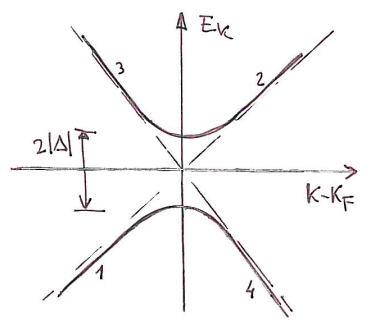
\includegraphics[width=0.4\linewidth]{Immagini - Capitolo 2/legge dispersione BCS.png}
    \caption{legge dispersione della teoria BCS dove le curve corrispondono all'energia di: 1. un quasi-elettrone con $k < k_F$; 2. un quasi-elettrone con $k > k_F$; una quasi-lacuna con $k < k_F$; 4. una quasi-lacuna con $k > k_F$.}
    \label{fig: legge dispersione BCS}
\end{figure}
Si intende adesso studiare l'andamento dei coefficienti
\begin{equation}
    |v_k|^2 = \frac{1}{2}\bigg(1 - \frac{\epsilon_k - \mu}{E_k}\bigg),\quad |u_k|^2 = \frac{1}{2}\bigg(1 + \frac{\epsilon_k - \mu}{E_k}\bigg),
\end{equation}
il cui andamento è mostrato in figura \ref{fig: coefficienti uk e vk}, dalla quale si nota che per $k - k_F \gg 0$ si hanno
\begin{align}
    \hatb_{k\upa} &= u_k^*\hatC_{k\upa} - v_k^*\hatCT_{-k\doa} \simeq u_k^*\hatC_{k\upa}, \\
    \hatbT_{-k\doa} &= v_k\hatC_{k\upa} + u_k\hatCT_{-k\doa} \simeq u_k\hatC_{-k\doa},
\end{align}
interpretati come gli operatori di distruzione e creazione di un quasi-elettrone rispettivamente, mentre per $k - k_F \ll 0$ si hanno
\begin{align}
    \hatb_{k\upa} &\simeq v_k^*\hatCT_{-k\doa}, \\
    \hatbT_{-k\doa} &\simeq v_k\hatC_{k\upa},
\end{align}
interpretati analogamente come gli operatori di distruzione e creazione di una quasi-lacuna rispettivamente. Quindi, gli operatori $\hatb$ e $\hatbT$ sono un mix di operatori di creazione di elettroni e lacune: gli stati che creano non sono né elettroni né lacune, ma una loro sovrapposizione quantistica. Dunque, i quasi-elettroni non hanno carica elettrica ben definita.
\begin{figure}[h]
    \centering
    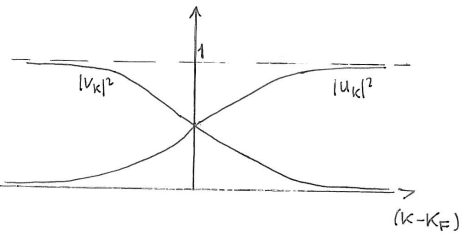
\includegraphics[width=0.5\linewidth]{Immagini - Capitolo 2/coefficienti uk e vk.png}
    \caption{andamento dei moduli $|u_k|^2$ e $|v_k|^2$ in funzione di $k - k_F$.}
    \label{fig: coefficienti uk e vk}
\end{figure}

Infatti, $u_k$ e $v_k$ hanno un'interpretazione probabilistica. Dato lo stato ad una particella
\begin{equation}
    \hatbT_{k\upa}\ket{\psi_{BCS}} = u_k\hatCT_{k\upa}\ket{\psi_{BCS}} - v_k\hatC_{-k\doa}\ket{\psi_{BCS}},
\end{equation}
il modulo $|u_k|^2$ è la probabilità di trovare un elettrone se si effettua una misura di carica, mentre $|v_k|^2$ è la probabilità di trovare una lacuna.
\begin{obs}
    Si ha un'interessante analogia con la fisica della particelle elementari. I mesoni $K^0$ e $\bar{K}^0$ sono formati da una coppia di quark $d\bar{s}$ e $s\bar{d}$, sono entrambi autostati dell'interazione forte e sono prodotti attraverso l'urto di protoni su un bersaglio, ma non sono autostati dell'interazione debole che non conserva la stranezza. Invece, si osservano oscillazioni tra uno stato e l'altro durante la propagazione.
\end{obs}

\subsection{Gap di energia}
A temperatura finita $T$, le quasi-particelle hanno numero di occupazione degli stati dato dalla distribuzione di Fermi-Dirac, ossia
\begin{equation}
    \vmedio{\hatbT_{k\upa}\hatb_{k\upa}}_T = \frac{1}{e^{\beta E_k} + 1} \equiv f(E_k)
\end{equation}
e di conseguenza
\begin{equation}
    \vmedio{\hatb_{-k\doa}\hatbT_{-k\doa}}_T = 1 - f(E_k).
\end{equation}
Per calcolare il valore di aspettazione $\vmedio{\hatC_{k\upa}\hatCT_{-k\doa}}_T$, si parte da
\begin{equation}
    \begin{pmatrix}
        \hatC_{k\upa} \\
        \hatCT_{-k\doa}
    \end{pmatrix} = U
    \begin{pmatrix}
        \hatb_{k\upa} \\
        \hatbT_{-k\doa}
    \end{pmatrix} = 
    \begin{pmatrix}
        u_k & v_k^* \\
        -v_k & u_k^*
    \end{pmatrix}
    \begin{pmatrix}
        \hatb_{k\upa} \\
        \hatbT_{-k\doa}
    \end{pmatrix},
\end{equation}
da cui si ha $\hatC_{-k\doa} = -v_k^*\hatbT_{k\upa} + u_k\hatb_{-k\doa}$, permettendo così di calcolare
\begin{equation}
    \begin{split}
        \vmedio{\hatC_{-k\doa}\hatC_{k\upa}}_T & =\vmedio{(-v_k^*\hatbT_{k\upa} + u_k\hatb_{-k\doa})(u_k\hatb_{k\upa} + v_k^*\hatbT_{-k\doa})}_T \\
        &= \vmedio{-v_k^*u_k\hatbT_{k\upa}\hatb_{k\upa} + u_kv_k^*\hatb_{-k\doa}\hatbT_{-k\doa}}_T \\
        &= v_k^*u_k[1 - 2f(E_k)].
    \end{split}
\end{equation}
Quindi, in funzione della temperatura il gap di energia è
\begin{equation}
    \Delta(T) = |g|\nsum_k\vmedio{\hatC_{k\upa}\hatC_{-k\doa}}_T = |g|\nsum_k u_kv_k^*[1 - 2f(E_k)],
\end{equation}
che generalizza il risultato per $T = \SI{0}{\kelvin}$. Dato che in prima approssimazione $u_kv_k^* = \Delta/2E_k$, allora
\begin{equation}
    \begin{split}
        \Delta(T) &= |g|\nsump{k}\frac{\Delta}{2E_k}\bigg(1 - \frac{2}{e^{\beta E_k} + 1}\bigg) \\
        &= |g|\nsump{k}\frac{\Delta}{2E_k}\frac{e^{\beta E_k/2} - e^{\beta E_k/2}}{e^{-\beta E_k/2} + e^{-\beta E_k/2}} \\
        &= g\nsump{k}\frac{\Delta}{2E_k}\tanh{\frac{E_k}{2kT}}.
    \end{split}
\end{equation}
Procedendo in modo simile al caso $T = \SI{0}{\kelvin}$, si ha
\begin{equation}
\label{eq: equazione del gap di energia BCS}
    \Lambda\int_0^{\hbar\omega_D}\frac{d\xi}{E(\xi)}\tanh{\frac{E(\xi)}{2kT}} = 1,\quad \xi \equiv \epsilon_k - \mu,
\end{equation}
dove $\Lambda = |g|D(\epsilon_F)$ e $E(\xi) = \sqrt{\xi^2 + |\Delta|^2}$.

\subsubsection{Dipendenza dalla temperatura}
Una stima della temperatura critica $T_c$ si ottiene sostituendo $T \to T_c$, per cui $\Delta(T_c) = 0$ e $E(\xi) = \xi$, nell'equazione \eqref{eq: equazione del gap di energia BCS}, ossia
\begin{equation}
    \Lambda\int_0^{\hbar\omega_D}\frac{d\xi}{\xi}\tanh{\frac{\xi}{2kT}} = \Lambda\int_0^{\beta\hbar\omega_D/2}\frac{dz}{z}\tanh{z},\quad z \equiv \frac{\xi}{2kT}.
\end{equation}
Per dare una stima dell'integrale 
\begin{equation}
    \int_0^y\frac{\tanh{z}}{z}\,dz,\quad y \gg 0,
\end{equation}
si integra per parti ottenendo
\begin{equation}
    \begin{split}
        \int_0^y\frac{\tanh{z}}{z}\,dz &= \log{(y)}\tanh{(y)} - \int_0^y\frac{\log{z}}{\cosh^2{z}}\,dz \\
        &\simeq \log{(y)} - \int_0^y\frac{\log{z}}{\cosh^2{z}}\,dz \\
        &= \log{(y)} - \bigg(-\gamma_E + \log{\frac{\pi}{4}}\bigg) \\
        &= \log{\bigg(\frac{\pi y}{4}e^{\gamma_E}\bigg)},
    \end{split}
\end{equation}
dove $\gamma_E = 0.577$ è la costante di Eulero-Mascheroni. Quindi, in questo caso
\begin{equation}
    \int_0^{\beta\hbar\omega_D/2}\frac{\tanh{z}}{z}\,dz \simeq \log{(A\hbar\omega_D\beta_C)},\quad A \equiv \frac{2e^{\gamma_E}}{\pi} \simeq 1.13,
\end{equation}
per cui 
\begin{equation}
    kT_c \simeq 1.13 \times (\hbar\omega_De^{-1/\Lambda}).
\end{equation}
Dunque, considerando il rapporto tra $\Delta(0) \simeq 2\hbar\omega_De^{-1/\Lambda}$ con $kT_c$ appena trovata si ha
\begin{equation}
    \frac{\Delta(0)}{kT_c} \simeq 1.76,
\end{equation}
che corrisponde ad una stima indipendente dal limite superiore $\hbar\omega_D$.
\begin{obs}
    Le quantità $\Delta(0)$ e $T_c$ possono essere misurate sperimentalmente in maniera indipendente. Il rapporto $\Delta(0)/kT_c$ misurato varia nel range $[1.6,2.3]$ nei superconduttori ``tradizionali'' con una distribuzione che si addensa intorno al valore teorico di 1.76.
\end{obs}
Per quanto riguarda $\Delta(T)$, questo può essere misurato numericamente dall'integrale
\begin{equation}
    \Lambda\int_0^{\hbar\omega_D}\frac{d\xi}{(\xi^2 + |\Delta|^2)^{1/2}}\tanh{\bigg[\frac{\beta}{2}(\xi^2 + |\Delta|^2)^{1/2}\bigg]} = 1.
\end{equation}
Per i superconduttori con $kT_c \ll \hbar\omega_D$, il rapporto $|\Delta(T)|/|\Delta(0)|$ è una funzione universale di $T/T_c$ che decresce monotonicamente da 1 a $T = \SI{0}{\kelvin}$ fino a zero per $T = T_c$. Intorno a $T = \SI{0}{\kelvin}$ la variazione è molto lenta poiché $e^{-\Delta/kT} \simeq 0$ e la tangente iperbolica è circa uno, quindi $\Delta(T)$ è circa costante fino a quando un grande numero di pseudo-particelle è stato eccitato termicamente. In particolare per $T \simeq T_c$, $\Delta(T)$ decresce a zero con tangente verticale 
\begin{equation}
    |\Delta(T)| \propto \bigg(1 - \frac{T}{T_c}\bigg)^{1/2}.
\end{equation}
\begin{obs}
    L'andamento con esponente critico pari ad $1/2$ è tipico di tutte le teorie di campo medio.
\end{obs}

\subsection{Densità degli stati}
Si può ottenere la densità degli stati $D_{BCS}$ nell'intorno dell'energia di Fermi come
\begin{equation}
    D_{BCS}(E)\,dE \simeq D(\epsilon_F)\,d(\epsilon - \mu) = D(\epsilon_F)\frac{d}{dE}(\epsilon - \mu)\,dE,
\end{equation}
dove 
\begin{equation}
    E(\epsilon - \mu) = 
    \begin{cases}
        -\sqrt{(\epsilon - \mu)^2 + |\Delta|^2},\quad \epsilon - \mu < 0 \\
        \sqrt{(\epsilon - \mu)^2 + |\Delta|^2},\quad \epsilon - \mu > 0
    \end{cases},
\end{equation}
la quale invertita restituisce
\begin{equation}
    \epsilon(E) - \mu = 
    \begin{cases}
        -\sqrt{E^2 - |\Delta|^2},\quad E < - |\Delta| \\
        0,\quad -|\Delta| \le E \le |\Delta| \\
        \sqrt{E^2 - |\Delta|^2},\quad E > |\Delta|
    \end{cases},
\end{equation}
la cui derivata è
\begin{equation}
    \frac{d}{dE}(\epsilon - \mu) = 
    \begin{cases}
        -\dfrac{E}{(E^2 - |\Delta|^2)^{1/2}},\quad E < - |\Delta| \\
        0,\quad -|\Delta| \le E \le |\Delta| \\
        \dfrac{E}{(E^2 - |\Delta|^2)^{1/2}},\quad E > |\Delta|
    \end{cases},
\end{equation}
dalla quale si può dedurre l'andamento della densità di stati $D_{BCS}$ mostrato in figura \ref{fig: densità di stati BCS}.
\begin{figure}[h]
    \centering
    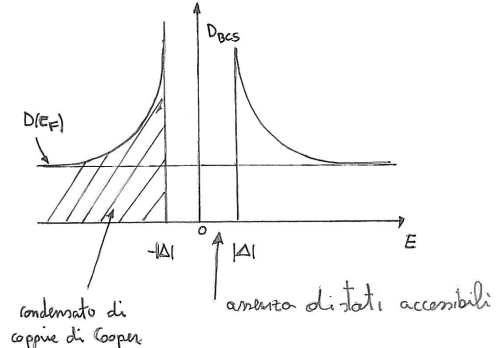
\includegraphics[width=0.4\linewidth]{Immagini - Capitolo 2/densità di stati BCS.png}
    \caption{andamento della densità di stati $D_{BCS}$ in funzione dell'energia.}
    \label{fig: densità di stati BCS}
\end{figure}

\subsection{scattering Andreev}
Un'ulteriore conferma dell'esistenza delle coppie di Cooper e del gap di energia si ottiene attraverso lo scattering di elettroni nel passaggio tra un metallo in regime classico e un altro in regime di superconduzione. Si consideri quindi un elettrone nel metallo in regime normale con impulso $\vk$, energia $\epsilon_k$ e terza componente di spin $\sigma$: se l'energia $\epsilon_k$ è minore di $|\Delta| + \epsilon_F$, allora l'elettrone non dovrebbe potersi propagare nel superconduttore, implicando quindi l'assenza di stati accessibili, e dovrebbe quindi essere riflesso all'interfaccia tra i due regimi, con il superconduttore che si comporta come un isolante. Si noti che nell'urto si conserva la carica elettrica, l'energia e lo spin, mentre non si conserva l'impulso.  
\begin{figure}[h]
    \centering
    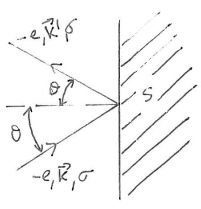
\includegraphics[width=0.3\linewidth]{Immagini - Capitolo 2/scattering C-SC.png}
    \caption{scattering di un elettrone all'interfaccia.}
    \label{fig: scattering C-SC}
\end{figure}

Tuttavia, Andreev osservò che nei superconduttori è possibile un altro processo: l'elettrone può combinarsi con un altro elettrone del metallo con impulso $\vk$ e spin $-\sigma$ per formare una coppia di Cooper che può propagarsi nel superconduttore sotto forma di supercorrente. Nel conduttore normale rimane però una lacuna con carica $e$, momento $\vk$, spin $\sigma$ e velocità di gruppo pari a 
\begin{equation}
    -\frac{\p}{\p\vk}\bigg(\frac{\hbar^2k^2}{2m} - \mu\bigg) = -\frac{\hbar^2}{2m}\vk.
\end{equation}
\begin{figure}[h]
    \centering
    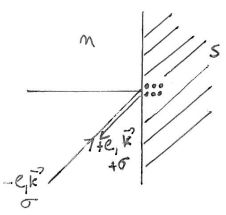
\includegraphics[width=0.3\linewidth]{Immagini - Capitolo 2/Andreev scattering.png}
    \caption{scattering Andreev.}
    \label{fig: Andreev scattering}
\end{figure}

Un'evidenza diretta di questo tipo di scattering si può ottenere iniettando una corrente all'interfaccia con un un superconduttore. Poiché la lacuna che torna indietro trasporta carica $e$, la corrente che passa nel superconduttore per effetto tunnel risulta essere il doppio rispetto a quella ottenibile per $\Delta = 0$ o per $\epsilon_k > |\Delta| + \epsilon_F$. La corrente trasportata dalla stato $\ket{\psi_{BCS}}$ è nulla; infatti calcolando il valore di aspettazione di $\hatJ_S$ si trova proprio
\begin{equation}
    \begin{split}
        \vJ_S = \mybrakett{\psi_{BCS}}{\hatJ_S}{\psi_{BCS}} &= \nsum_k\frac{\hbar}{2m}\vk(\vmedio{\hatN_{k\upa}}_{BCS} - \vmedio{\hatN_{-k\doa}}_{BCS}) \\
        &= \nsum_k\frac{\hbar}{m}\vk(|v_k|^2 - |v_k|^2) \\
        &= 0.
    \end{split}
\end{equation}
Bisognerebbe dimostrare che il gap di energia esiste anche quando le coppie di Cooper si muovono collettivamente, ossia per $\ket{\psi_{BCS}} \to \ket{\psi_{BCS},\vQ}$, dove 
\begin{equation}
    \ket{\psi_{BCS},\vQ} = \nprod_k(u_k^* + v_k^*\hatCT_{k + Q,\upa}\hatCT_{-k + Q,\doa})\kO.
\end{equation}
Questo stato corrisponde ad una soluzione consistente nel tempo di campo medio dell'hamiltoniana del modello BCS con 
\begin{align}
    \Delta Q &= |g|\nsum_k\vmedio{\hatC_{-k + Q,\doa}\hatC_{k + Q,\upa}}_{BCS}, \\
    \Delta^* Q &= |g|\nsum_k\vmedio{\hatCT_{-k + Q,\upa}\hatCT_{-k + Q,\doa}}_{BCS}.
\end{align}
L'hamiltoniana risultante può essere diagonalizzata e le eccitazioni di quasi-elettroni sopra questo stato possiedono una legge di dispersione ``deformata'', ma c'è ancora un gap di energia pari a 
\begin{equation}
    \Delta E \simeq 2|\Delta(0)| - \frac{2\hbar^2Qk_F}{m}.
\end{equation}